\documentclass{article} % use larger type; default would be 10pt

\usepackage{tikz}
\usepackage{pgfplots}
\usetikzlibrary{calc}
\usetikzlibrary{arrows}
\usetikzlibrary{patterns}
\usetikzlibrary{calc,intersections,through,backgrounds}
\usetikzlibrary{decorations.pathreplacing}
        \newcommand\degree[0]{^{\circ}}
        \newcommand\abs[1]{\left|#1\right|}

\title{Play with TikZ}
\author{Just Us}
%\date{} % Activate to display a given date or no date (if empty),
         % otherwise the current date is printed 

\begin{document}
\maketitle

\section{Chapter 8 Section 3}

For first image use fig-4-2-caut1 


exam8-3-1 angle

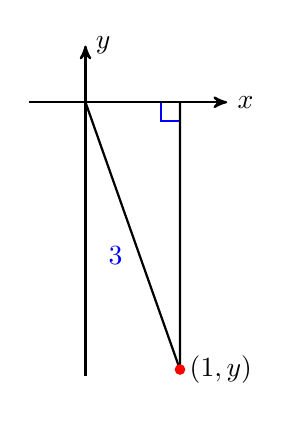
\begin{tikzpicture} [scale=1.2]
\draw[blue,thick] (1,0) rectangle ++(-.2,-.2);
\draw[black,thick,->,>=stealth'] (-.6,0)--(1.5,0) node[right] {$x$};
\draw[black,thick,->,>=stealth'] (0,-2.9)--(0,.6) node[right] {$y$};
\coordinate (P) at ({-acos(1/3)}:3);
\draw[black,thick] (0,0)--(P) node[below left, midway, text=blue] {$3$};
\draw[black,thick] (1,0)--(P);
\filldraw[red] (P) circle (.05cm) node[right, text=black] {$(1,y)$};
\end{tikzpicture}
\newline

exam8-3-4 shadow of flagpole

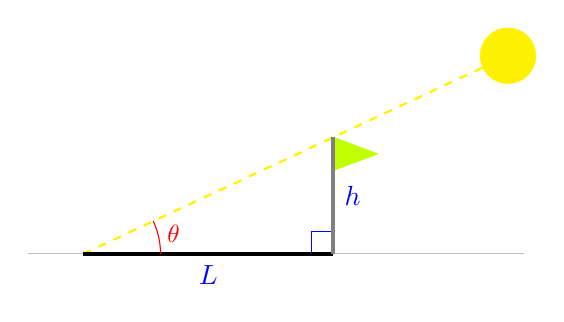
\begin{tikzpicture} [scale=1.4]
\def\th{25};
\def\ra{2.5};
\coordinate(O) at (0,0);
\coordinate (A) at ($ \ra*cos(\th)*(1,0) $);
\coordinate (B) at ($ ({\th}:{\ra}) $);
\coordinate (C) at ($ ({\th}:{1.7*\ra}) $);
\draw[blue] (A) rectangle ++(-.2,.2);
\filldraw[lime] (B) -- ++(.4,-.15) --++(-.4,-.15)--++(0,.3);
\draw[lightgray] (-.5,0)--(4,0);
\draw[yellow, thick, dashed] (O)--(C);
\draw[black,ultra thick] (O)--(A) node[below, midway, text=blue] {$L$};
\draw[gray, ultra thick] (A)--(B) node[right, midway, text=blue] {$h$};
\filldraw[yellow] (C) circle (.25cm);
\draw[red] (0.7,0) arc(0:{\th}:0.7) node[right, midway, yshift=1, scale=.9] {$\theta$};
\end{tikzpicture}
\newline

exer8-3-4 hexagon (regular polygon)

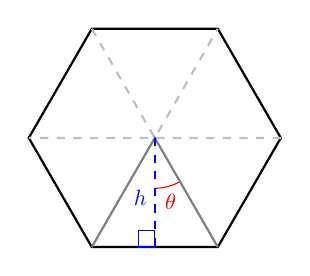
\begin{tikzpicture} [scale=1.6]
\def\th{60};
\coordinate(O) at (0,0);
\coordinate (A) at (1,0);
\coordinate (B) at ({\th}:1);
\coordinate (C) at ({2*\th}:1);
\coordinate (D) at ({3*\th}:1);
\coordinate (E) at ({4*\th}:1);
\coordinate (F) at ({5*\th}:1);
\draw[black,thick] (A)--(B)--(C)--(D)--(E)--(F)--(A);
\draw[lightgray,thick,dashed] (A)--(O)--(B);
\draw[lightgray,thick,dashed] (C)--(O)--(D);
\draw[red] (0,-.4) arc(-90:-60:.4) node[below, xshift=1, midway, scale=.8] {$\theta$};
\draw[gray,thick] (F)--(O)--(E);
\coordinate (P) at ($ cos(\th /2) *(0,-1) $);
\draw[blue] (P) rectangle ++(-.13,.13);
\draw[blue,thick, dashed] (O)--(P) node[left, yshift=-2,midway, scale=.8] {$h$};
\end{tikzpicture}
\newline

exam8-3-5a cosine

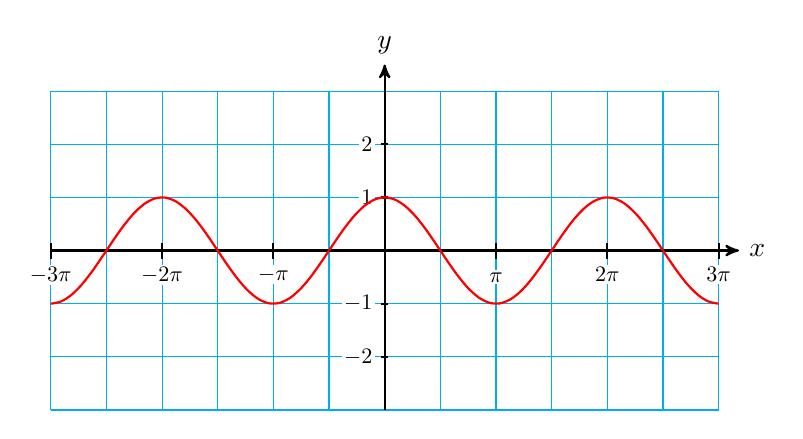
\begin{tikzpicture} [xscale=.45, yscale=.675]
\draw[cyan] (-3*pi,-3) grid[xstep=pi/2] (3*pi,3);
\draw[black,thick,->,>=stealth'] (-3*pi,0)--(10,0) node[right] {$x$};
\draw[black,thick,->,>=stealth'] (0,-3)--(0,3.5) node[above] {$y$};
\foreach \y in {-2,-1,1,2} \draw[black,thick] (.1,\y)--++(-.2,0) node [left, xshift=-2, fill=white, inner sep=1, scale=.8] {$\y$};
\foreach \x [evaluate=\x as \xp using (pi*\x)] in {2,3} {
  \draw[black,thick] (\xp,0.15)--++(0,-.3) node[below, yshift=-2, fill=white, inner sep=1, scale=.8] {$\x \pi$};
  \draw[black,thick] (-\xp,0.15)--++(0,-.3) node[below, yshift=-2, fill=white, inner sep=1, scale=.8] {$-\x \pi$};
};
\draw[black,thick] (-pi,0.15)--++(0,-.3) node[below, yshift=-2, fill=white, inner sep=1, scale=.8] {$-\pi$};
\draw[black,thick] (pi,0.15)--++(0,-.3) node[below, yshift=-4, fill=white, inner sep=1, scale=.8] {$\pi$};
\draw[samples=65, domain=-3*pi:3*pi, variable=\x, smooth, red, thick] plot (\x, {cos(deg(\x))});
\end{tikzpicture}
\newline

exam8-3-5b grid

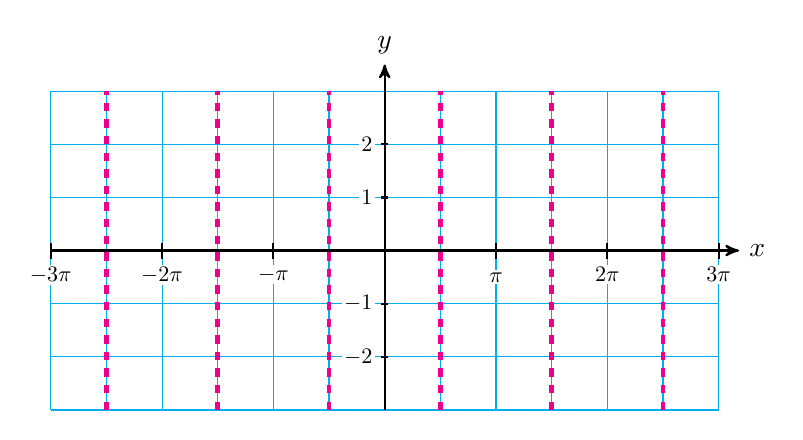
\begin{tikzpicture} [xscale=.45, yscale=.675]
\draw[cyan] (-3*pi,-3) grid[xstep=pi/2] (3*pi,3);
\draw[black,thick,->,>=stealth'] (-3*pi,0)--(10,0) node[right] {$x$};
\draw[black,thick,->,>=stealth'] (0,-3)--(0,3.5) node[above] {$y$};
\foreach \y in {-2,-1,1,2} \draw[black,thick] (.1,\y)--++(-.2,0) node [left, xshift=-2, fill=white, inner sep=1, scale=.8] {$\y$};
\foreach \x [evaluate=\x as \xp using (pi*\x)] in {2,3} {
  \draw[black,thick] (\xp,0.15)--++(0,-.3) node[below, yshift=-2, fill=white, inner sep=1, scale=.8] {$\x \pi$};
  \draw[black,thick] (-\xp,0.15)--++(0,-.3) node[below, yshift=-2, fill=white, inner sep=1, scale=.8] {$-\x \pi$};
};
\draw[black,thick] (-pi,0.15)--++(0,-.3) node[below, yshift=-2, fill=white, inner sep=1, scale=.8] {$-\pi$};
\draw[black,thick] (pi,0.15)--++(0,-.3) node[below, yshift=-4, fill=white, inner sep=1, scale=.8] {$\pi$};
\foreach \x [evaluate=\x as \xp using (pi*\x/2)] in {1,3,5} {
  \draw[magenta,ultra thick,dashed] (\xp,-3)--++(0,6);
  \draw[magenta,ultra thick,dashed] (-\xp,-3)--++(0,6);
};
 
\end{tikzpicture}
\newline

exam8-3-5ans cosine and secant

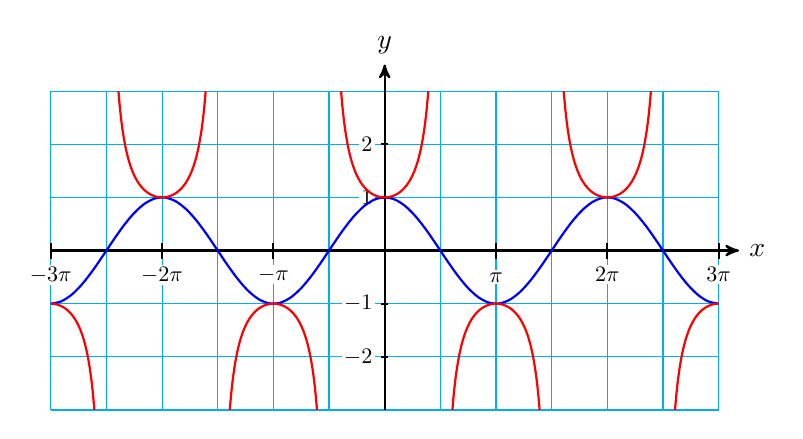
\begin{tikzpicture} [xscale=.45, yscale=.675]
\draw[cyan] (-3*pi,-3) grid[xstep=pi/2] (3*pi,3);
\draw[black,thick,->,>=stealth'] (-3*pi,0)--(10,0) node[right] {$x$};
\draw[black,thick,->,>=stealth'] (0,-3)--(0,3.5) node[above] {$y$};
\foreach \y in {-2,-1,1,2} \draw[black,thick] (.1,\y)--++(-.2,0) node [left, xshift=-2, fill=white, inner sep=1, scale=.8] {$\y$};
\foreach \x [evaluate=\x as \xp using (pi*\x)] in {2,3} {
  \draw[black,thick] (\xp,0.15)--++(0,-.3) node[below, yshift=-2, fill=white, inner sep=1, scale=.8] {$\x \pi$};
  \draw[black,thick] (-\xp,0.15)--++(0,-.3) node[below, yshift=-2, fill=white, inner sep=1, scale=.8] {$-\x \pi$};
};
\draw[black,thick] (-pi,0.15)--++(0,-.3) node[below, yshift=-2, fill=white, inner sep=1, scale=.8] {$-\pi$};
\draw[black,thick] (pi,0.15)--++(0,-.3) node[below, yshift=-4, fill=white, inner sep=1, scale=.8] {$\pi$};
\draw[samples=65, domain=-3*pi:3*pi, variable=\x, smooth, blue, thick] plot (\x, {cos(deg(\x))});
\draw[samples=65, domain={-acos(1/3)*pi/180}:{acos(1/3)*pi/180}, variable=\x, smooth, red, thick] plot ({\x-2*pi}, {sec(deg(\x))});
\draw[samples=65, domain={-acos(1/3)*pi/180}:{acos(1/3)*pi/180}, variable=\x, smooth, red, thick] plot (\x, {sec(deg(\x))});
\draw[samples=65, domain={-acos(1/3)*pi/180}:{acos(1/3)*pi/180}, variable=\x, smooth, red, thick] plot ({\x+2*pi}, {sec(deg(\x))});
\draw[samples=65, domain={-acos(1/3)*pi/180}:{acos(1/3)*pi/180}, variable=\x, smooth, red, thick] plot ({\x-pi}, {-sec(deg(\x))});
\draw[samples=65, domain={-acos(1/3)*pi/180}:{acos(1/3)*pi/180}, variable=\x, smooth, red, thick] plot ({\x+pi}, {-sec(deg(\x))});

\draw[samples=65, domain=0:{acos(1/3)*pi/180}, variable=\x, smooth, red, thick] plot ({\x-3*pi}, {-sec(deg(\x))});
\draw[samples=65, domain={-acos(1/3)*pi/180}:{0}, variable=\x, smooth, red, thick] plot ({\x+3*pi}, {-sec(deg(\x))});
\end{tikzpicture}
\newline

exam8-3-5ans tan and cotan

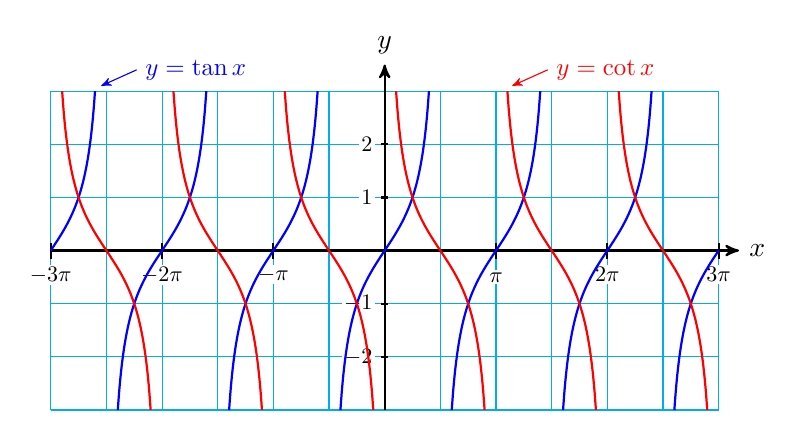
\begin{tikzpicture} [xscale=.45, yscale=.675]
\draw[cyan] (-3*pi,-3) grid[xstep=pi/2] (3*pi,3);
\draw[black,thick,->,>=stealth'] (-3*pi,0)--(10,0) node[right] {$x$};
\draw[black,thick,->,>=stealth'] (0,-3)--(0,3.5) node[above] {$y$};
\foreach \y in {-2,-1,1,2} \draw[black,thick] (.1,\y)--++(-.2,0) node [left, xshift=-2, fill=white, inner sep=1, scale=.8] {$\y$};
\foreach \x [evaluate=\x as \xp using (pi*\x)] in {2,3} {
  \draw[black,thick] (\xp,0.15)--++(0,-.3) node[below, yshift=-2, fill=white, inner sep=1, scale=.8] {$\x \pi$};
  \draw[black,thick] (-\xp,0.15)--++(0,-.3) node[below, yshift=-2, fill=white, inner sep=1, scale=.8] {$-\x \pi$};
};
\draw[black,thick] (-pi,0.15)--++(0,-.3) node[below, yshift=-2, fill=white, inner sep=1, scale=.8] {$-\pi$};
\draw[black,thick] (pi,0.15)--++(0,-.3) node[below, yshift=-4, fill=white, inner sep=1, scale=.8] {$\pi$};

\draw[samples=65, domain={0}:{atan(3)*pi/180}, variable=\x, smooth, blue, thick] plot ({\x-3*pi}, {tan(deg(\x))});
\draw[samples=65, domain={-atan(3)*pi/180}:{atan(3)*pi/180}, variable=\x, smooth, blue, thick] plot ({\x-2*pi}, {tan(deg(\x))});
\draw[samples=65, domain={-atan(3)*pi/180}:{atan(3)*pi/180}, variable=\x, smooth, blue, thick] plot (\x, {tan(deg(\x))});
\draw[samples=65, domain={-atan(3)*pi/180}:{atan(3)*pi/180}, variable=\x, smooth, blue, thick] plot ({\x+2*pi}, {tan(deg(\x))});
\draw[samples=65, domain={-atan(3)*pi/180}:{atan(3)*pi/180}, variable=\x, smooth, blue, thick] plot ({\x-pi}, {tan(deg(\x))});
\draw[samples=65, domain={-atan(3)*pi/180}:{atan(3)*pi/180}, variable=\x, smooth, blue, thick] plot ({\x+pi}, {tan(deg(\x))});
\draw[samples=65, domain={-atan(3)*pi/180}:{0}, variable=\x, smooth, blue, thick] plot ({\x+3*pi}, {tan(deg(\x))});

\draw[samples=65, domain={-atan(3)*pi/180}:{atan(3)*pi/180}, variable=\x, smooth, red, thick] plot ({\x-5/2*pi}, {-tan(deg(\x))});
\draw[samples=65, domain={-atan(3)*pi/180}:{atan(3)*pi/180}, variable=\x, smooth, red, thick] plot ({\x-pi/2}, {-tan(deg(\x))});
\draw[samples=65, domain={-atan(3)*pi/180}:{atan(3)*pi/180}, variable=\x, smooth, red, thick] plot ({\x+3/2*pi}, {-tan(deg(\x))});
\draw[samples=65, domain={-atan(3)*pi/180}:{atan(3)*pi/180}, variable=\x, smooth, red, thick] plot ({\x-3/2*pi}, {-tan(deg(\x))});
\draw[samples=65, domain={-atan(3)*pi/180}:{atan(3)*pi/180}, variable=\x, smooth, red, thick] plot ({\x+1/2*pi}, {-tan(deg(\x))});
\draw[samples=65, domain={-atan(3)*pi/180}:{atan(3)*pi/180}, variable=\x, smooth, red, thick] plot ({\x+5/2*pi}, {-tan(deg(\x))});
\draw[blue,<-,>=stealth'] (-8,3.1)--++(1,.3) node[ right, scale=.9] {$y=\tan x$};
\draw[red,<-,>=stealth'] (3.6,3.1)--++(1,.3) node[ right, scale=.9] {$y=\cot x$};
\end{tikzpicture}
\newline

fig-8-3-2 three reciprocal trig functions

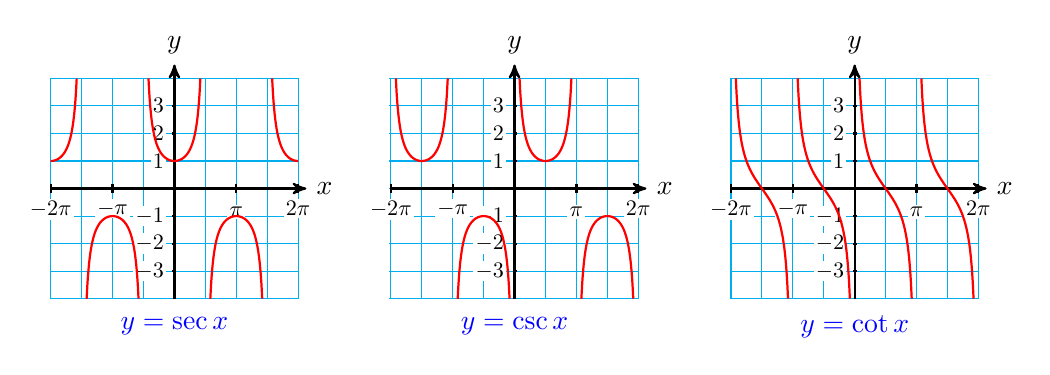
\begin{tikzpicture} [xscale=.25, yscale=.35]
\draw[cyan] (-2*pi,-4) grid[xstep=pi/2] (2*pi,4);
\draw[black,thick,->,>=stealth'] (-2*pi,0)--(6.7,0) node[right] {$x$};
\draw[black,thick,->,>=stealth'] (0,-4)--(0,4.5) node[above] {$y$};
\foreach \y in {-2,-1,1,2, -3,3} \draw[black,thick] (.1,\y)--++(-.2,0) node [left, xshift=-2, fill=white, inner sep=1, scale=.8] {$\y$};
\foreach \x [evaluate=\x as \xp using (pi*\x)] in {2} {
  \draw[black,thick] (\xp,0.15)--++(0,-.3) node[below, yshift=-2, fill=white, inner sep=1, scale=.8] {$\x \pi$};
  \draw[black,thick] (-\xp,0.15)--++(0,-.3) node[below, yshift=-2, fill=white, inner sep=1, scale=.8] {$-\x \pi$};
};
\draw[black,thick] (-pi,0.15)--++(0,-.3) node[below, yshift=-2, fill=white, inner sep=1, scale=.8] {$-\pi$};
\draw[black,thick] (pi,0.15)--++(0,-.3) node[below, yshift=-4, fill=white, inner sep=1, scale=.8] {$\pi$};
\draw[samples=65, domain={0}:{acos(1/4)*pi/180}, variable=\x, smooth, red, thick] plot ({\x-2*pi}, {sec(deg(\x))});
\draw[samples=65, domain={-acos(1/4)*pi/180}:{acos(1/4)*pi/180}, variable=\x, smooth, red, thick] plot (\x, {sec(deg(\x))});
\draw[samples=65, domain={-acos(1/4)*pi/180}:{0}, variable=\x, smooth, red, thick] plot ({\x+2*pi}, {sec(deg(\x))});
\draw[samples=65, domain={-acos(1/4)*pi/180}:{acos(1/4)*pi/180}, variable=\x, smooth, red, thick] plot ({\x-pi}, {-sec(deg(\x))});
\draw[samples=65, domain={-acos(1/4)*pi/180}:{acos(1/4)*pi/180}, variable=\x, smooth, red, thick] plot ({\x+pi}, {-sec(deg(\x))});
\node[text=blue] at (0,-5.) {$y=\sec x$};

%second graph: cosecant
\def\de{11/2*pi}
\draw[cyan] (10.9,-4) grid[xstep=pi/2] ($ \de*(1,0)+(2*pi,4) $);
\draw[black,thick,->,>=stealth'] ($ \de*(1,0)+(-2*pi,0)$)--($ \de*(1,0)+(6.7,0)$) node[right] {$x$};
\draw[black,thick,->,>=stealth'] ($ \de*(1,0)+(0,-4)$)--($ \de*(1,0)+(0,4.5)$) node[above] {$y$};
\foreach \y in {-2,-1,1,2, -3,3} \draw[black,thick] ($ \de*(1,0)+(.1,\y)$)--++(-.2,0) node [left, xshift=-2, fill=white, inner sep=1, scale=.8] {$\y$};
\foreach \x [evaluate=\x as \xp using (pi*\x)] in {2} {
  \draw[black,thick] ($ \de*(1,0)+(\xp,0.15)$)--++(0,-.3) node[below, yshift=-2, fill=white, inner sep=1, scale=.8] {$\x \pi$};
  \draw[black,thick] ($ \de*(1,0)+(-\xp,0.15)$)--++(0,-.3) node[below, yshift=-2, fill=white, inner sep=1, scale=.8] {$-\x \pi$};
};
\draw[black,thick] ($ \de*(1,0)+(-pi,0.15)$)--++(0,-.3) node[below, yshift=-2, fill=white, inner sep=1, scale=.8] {$-\pi$};
\draw[black,thick] ($ \de*(1,0)+(pi,0.15)$)--++(0,-.3) node[below, yshift=-4, fill=white, inner sep=1, scale=.8] {$\pi$};

\draw[samples=65, domain={-acos(1/4)*pi/180}:{acos(1/4)*pi/180}, variable=\x, smooth, red, thick] plot (\x+\de-3*pi/2, {sec(deg(\x))});
\draw[samples=65, domain={-acos(1/4)*pi/180}:{acos(1/4)*pi/180}, variable=\x, smooth, red, thick] plot (\x+\de+pi/2, {sec(deg(\x))});
\draw[samples=65, domain={-acos(1/4)*pi/180}:{acos(1/4)*pi/180}, variable=\x, smooth, red, thick] plot ({\x-pi+\de+pi/2}, {-sec(deg(\x))});
\draw[samples=65, domain={-acos(1/4)*pi/180}:{acos(1/4)*pi/180}, variable=\x, smooth, red, thick] plot ({\x+3*pi/2+\de}, {-sec(deg(\x))});
\node[text=blue] at ($ \de*(1,0)+(0,-5.)$) {$y=\csc x$};


%third graph: cotangent
\def\de{11*pi}
\draw[cyan] (28.2,-4) grid[xstep=pi/2] ($ \de*(1,0)+(2*pi,4) $);
\draw[black,thick,->,>=stealth'] ($ \de*(1,0)+(-2*pi,0)$)--($ \de*(1,0)+(6.7,0)$) node[right] {$x$};
\draw[black,thick,->,>=stealth'] ($ \de*(1,0)+(0,-4)$)--($ \de*(1,0)+(0,4.5)$) node[above] {$y$};
\foreach \y in {-2,-1,1,2, -3,3} \draw[black,thick] ($ \de*(1,0)+(.1,\y)$)--++(-.2,0) node [left, xshift=-2, fill=white, inner sep=1, scale=.8] {$\y$};
\foreach \x [evaluate=\x as \xp using (pi*\x)] in {2} {
  \draw[black,thick] ($ \de*(1,0)+(\xp,0.15)$)--++(0,-.3) node[below, yshift=-2, fill=white, inner sep=1, scale=.8] {$\x \pi$};
  \draw[black,thick] ($ \de*(1,0)+(-\xp,0.15)$)--++(0,-.3) node[below, yshift=-2, fill=white, inner sep=1, scale=.8] {$-\x \pi$};
};
\draw[black,thick] ($ \de*(1,0)+(-pi,0.15)$)--++(0,-.3) node[below, yshift=-2, fill=white, inner sep=1, scale=.8] {$-\pi$};
\draw[black,thick] ($ \de*(1,0)+(pi,0.15)$)--++(0,-.3) node[below, yshift=-4, fill=white, inner sep=1, scale=.8] {$\pi$};

\draw[samples=65, domain={-atan(4)*pi/180}:{atan(4)*pi/180}, variable=\x, smooth, red, thick] plot (\x+\de-3*pi/2, {-tan(deg(\x))});
\draw[samples=65, domain={-atan(4)*pi/180}:{atan(4)*pi/180}, variable=\x, smooth, red, thick] plot (\x+\de+pi/2, {-tan(deg(\x))});
\draw[samples=65, domain={-atan(4)*pi/180}:{atan(4)*pi/180}, variable=\x, smooth, red, thick] plot ({\x-pi+\de+pi/2}, {-tan(deg(\x))});
\draw[samples=65, domain={-atan(4)*pi/180}:{atan(4)*pi/180}, variable=\x, smooth, red, thick] plot ({\x+3*pi/2+\de}, {-tan(deg(\x))});
\node[text=blue] at ($ \de*(1,0)+(0,-5.)$) {$y=\cot x$};

\end{tikzpicture}
\newline

fig-8-3-act1 unit circle and trig ratios

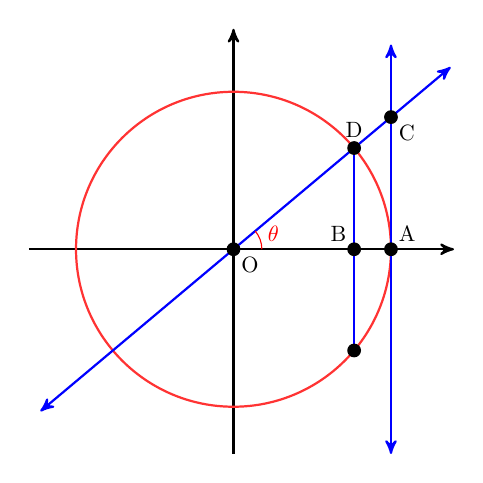
\begin{tikzpicture} [scale=2]
\coordinate (O) at (0,0);
\coordinate (A) at (1,0);
\def\th{40};
\coordinate (B) at ($ cos(\th)*(1,0)$);
\coordinate (C) at ($ tan(\th)*(0,1)+(1,0)$);
\coordinate (D) at ({\th}:1);
\coordinate (E) at ({-\th}:1);

\def\dx{1.3}
\draw[black,thick,->,>=stealth'] (-\dx,0)--(1.4,0);
\draw[black,thick,->,>=stealth'] (0,-\dx)--(0,1.4);
\draw[red!80!white,thick] (O) circle (1cm);

\draw[blue,thick] (D)--(E);
\draw[blue,thick,<->,>=stealth'] ({\th}:1.8)--({180+\th}:1.6);
\draw[blue,thick,<->,>=stealth'] (1,\dx)--(1,-\dx);

\filldraw[black] (O) circle (.04cm) node[below right, scale=.8]{O};
\filldraw[black] (A) circle (.04cm) node[above right, scale=.8]{A};
\filldraw[black] (B) circle (.04cm) node[above left, scale=.8]{B};
\filldraw[black] (C) circle (.04cm) node[below right, scale=.8]{C};
\filldraw[black] (D) circle (.04cm) node[above, yshift=1, scale=.8]{D};
\filldraw[black] (E) circle (.04cm);
\draw[red] (0.18,0) arc(0:{\th}:0.18) node[right, midway, yshift=2, text=red, scale=.8] {$\theta$};

\end{tikzpicture}
\newline

fig-8-3-act2 unit circle and trig ratios

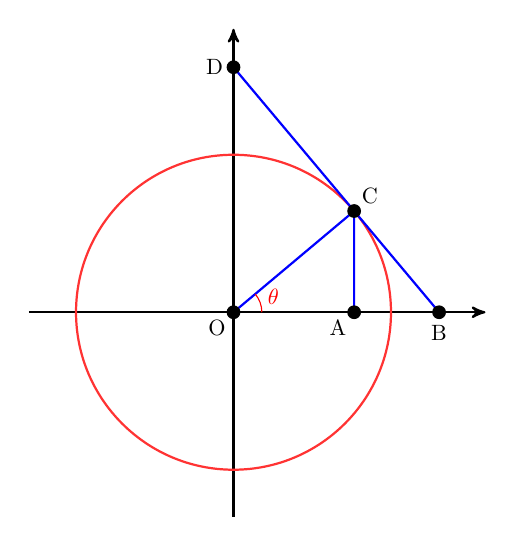
\begin{tikzpicture} [scale=2]
\coordinate (O) at (0,0);
\def\th{40};
\coordinate (A) at ($ cos(\th)*(1,0)$);
\coordinate (B) at ($ 1/cos(\th)*(1,0)$);
\coordinate (C) at ({\th}:1);
\coordinate (D) at ($ 1/sin(\th)*(0,1)$);

\def\dx{1.3}
\draw[black,thick,->,>=stealth'] (-\dx,0)--(1.6,0);
\draw[black,thick,->,>=stealth'] (0,-\dx)--(0,1.8);
\draw[red!80!white,thick] (O) circle (1cm);

\draw[blue,thick] (D)--(B);
\draw[blue,thick] (O)--(C)--(A);

\filldraw[black] (O) circle (.04cm) node[below left, scale=.8]{O};
\filldraw[black] (A) circle (.04cm) node[below left, scale=.8]{A};
\filldraw[black] (B) circle (.04cm) node[below, yshift=-2, scale=.8]{B};
\filldraw[black] (C) circle (.04cm) node[above right, scale=.8]{C};
\filldraw[black] (D) circle (.04cm) node[left, xshift=-1, scale=.8]{D};
\draw[red] (0.18,0) arc(0:{\th}:0.18) node[right, midway, yshift=2, text=red, scale=.8] {$\theta$};

\end{tikzpicture}
\newline

ar8-3-7ans $\frac{x}{\abs{x}}$

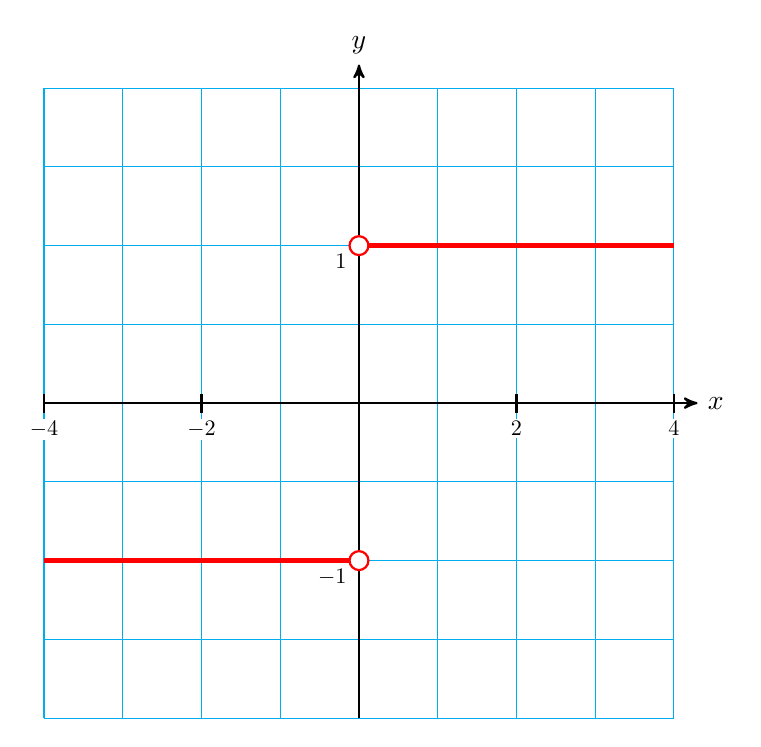
\begin{tikzpicture} [yscale=2]
\draw[cyan] (-4,-2) grid [ystep=1/2] (4,2);
\draw[black,thick,->,>=stealth'] (-4,0)--(4.3,0) node[right] {$x$};
\draw[black,thick,->,>=stealth'] (0,-2)--(0,2.15) node[above] {$y$};
\foreach \x in {-2,2,-4,4} \draw[black,thick] (\x,.06)--++(0,-.12) node[below, yshift=-2, fill=white, inner sep =1, scale=.8] {$\x$};
\foreach \y in {-1,1} \draw[black,thick] (.12,\y)--++(-.24,0) node[below left, yshift=-2, fill=white, inner sep =1, scale=.8] {$\y$};
\draw[red, ultra thick] (0,1)--(4,1);
\draw[red, ultra thick] (0,-1)--(-4,-1);
\draw[red, thick, fill=white] (0,1) ellipse (.12cm and .06 cm);
\draw[red, thick, fill=white] (0,-1) ellipse (.12cm and .06 cm);
\end{tikzpicture}
\newline


hp8-3-21 3-4-5 triangle

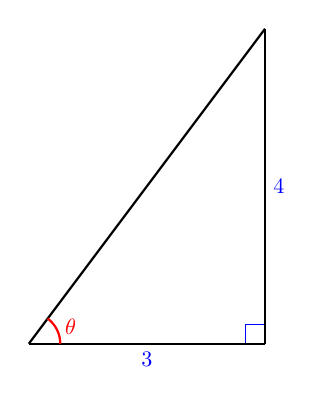
\begin{tikzpicture}
\coordinate (O) at (0,0);
\coordinate (A) at (3,0);
\coordinate (B) at (3,4);
\draw[blue] (A) rectangle ++(-.25,.25);
\draw[black,thick] (O)--(B);
\draw[black,thick] (O)--(A) node[below, midway,scale=.8, text=blue] {$3$};
\draw[black,thick] (B)--(A) node[right, midway,scale=.8, text=blue] {$4$};
\draw[red,thick] (0.4,0) arc(0: {atan(4/3)}:0.4) node[right, midway, yshift=1, scale=.8] {$\theta$};

\end{tikzpicture}
\newline


hp8-3-22  triangle

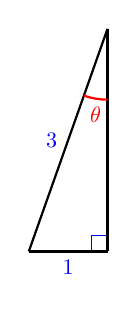
\begin{tikzpicture}
\coordinate (O) at (0,0);
\coordinate (A) at (1,0);
\coordinate (B) at ($ sqrt(8)*(0,1) + (1,0)$);
\draw[blue] (A) rectangle ++(-.2,.2);
\draw[black,thick] (A)--(B);
\draw[black,thick] (O)--(A) node[below, midway,scale=.8, text=blue] {$1$};
\draw[black,thick] (B)--(O) node[left, xshift=-1, midway,scale=.8, text=blue] {$3$};
\draw[red,thick] ({acos(1/3)}:2.1 ) arc({180+acos(1/3)}:270:0.9) node[below, midway, scale=.8] {$\theta$};

\end{tikzpicture}
\newline


hp8-3-23  triangle

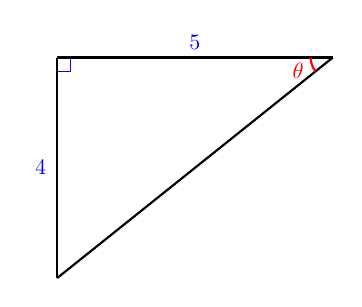
\begin{tikzpicture} [scale=.7]
\coordinate (O) at (0,0);
\coordinate (A) at (5,0);
\coordinate (B) at (0,-4);
\draw[blue] (O) rectangle ++(.25,-.25);
\draw[black,thick] (A)--(B);
\draw[black,thick] (O)--(A) node[above, midway,scale=.8, text=blue] {$5$};
\draw[black,thick] (B)--(O) node[left, xshift=-1, midway,scale=.8, text=blue] {$4$};
\draw[red,thick] (4.6,0 ) arc(180:{180+atan(4/5)}:0.4) node[left, midway, yshift=-2, scale=.8] {$\theta$};

\end{tikzpicture}
\newline


hp8-3-24  triangle

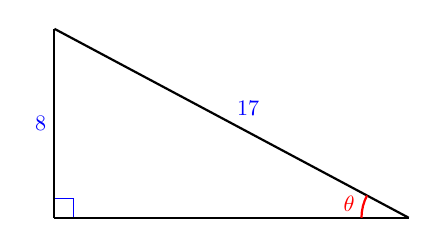
\begin{tikzpicture} [scale=.3]
\coordinate (O) at (0,0);
\coordinate (A) at (-15,0);
\coordinate (B) at (-15,8);
\draw[blue] (A) rectangle ++(.8,.8);
\draw[black,thick] (A)--(O);
\draw[black,thick] (B)--(A) node[left, midway,scale=.8, text=blue] {$8$};
\draw[black,thick] (B)--(O) node[above right, xshift=-1, midway,scale=.8, text=blue] {$17$};
\draw[red,thick] (-2,0 ) arc(180:{180-atan(8/15)}:2) node[left, midway, yshift=1, scale=.8] {$\theta$};

\end{tikzpicture}
\newline


hp8-3-25  angle

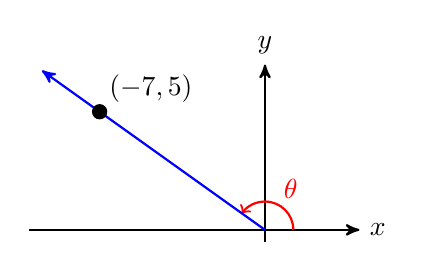
\begin{tikzpicture} [scale=.3]
\coordinate (O) at (0,0);
\coordinate (A) at (-7,5);
\draw[black,thick,->,>=stealth'] (-10,0)--(4,0) node[right]{$x$};
\draw[black,thick,->,>=stealth'] (0,-.5)--(0,7) node[above]{$y$};
\draw[red,thick, ->] (1.2,0 ) arc(0:{180-atan(5/7)}:1.2) node[above right, midway, yshift=-2,] {$\theta$};
\draw[blue,thick] (O)--(A);
\draw[blue,thick,->,>=stealth'] (A)--++({180-atan(5/7)}:3);
\filldraw[black] (A) circle (.3cm) node[above right] {$(-7,5)$};

\end{tikzpicture}
\newline


hp8-3-26  angle

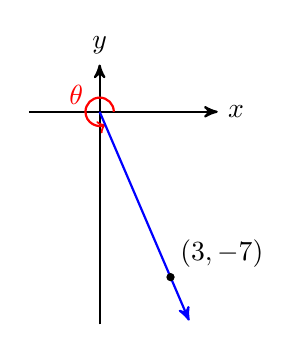
\begin{tikzpicture} [scale=.3]
\coordinate (O) at (0,0);
\coordinate (A) at (3,-7);
\draw[black,thick,->,>=stealth'] (-3,0)--(5,0) node[right]{$x$};
\draw[black,thick,->,>=stealth'] (0,-9)--(0,2) node[above]{$y$};
\draw[red,thick, ->] (0.6,0 ) arc(0:{360-atan(7/3)}:0.6) node[above left, midway, yshift=-4, xshift=2,] {$\theta$};
\draw[blue,thick] (O)--(A);
\draw[blue,thick,->,>=stealth'] (A)--++({360-atan(7/3)}:2);
\filldraw[black] (A) circle (.15cm) node[above right] {$(3,-7)$};

\end{tikzpicture}
\newline


hp8-3-27  angle

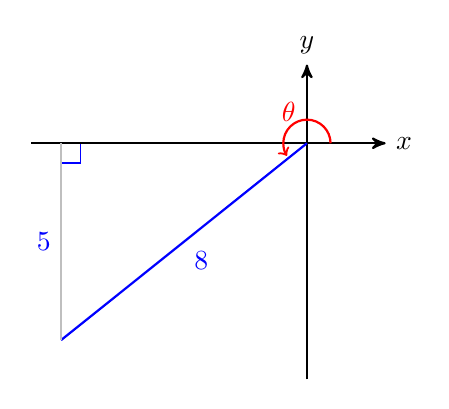
\begin{tikzpicture} [scale=.5]
\coordinate (O) at (0,0);
\coordinate (A) at ($ sqrt(39)*(-1,0) +(0,-5) $);
\coordinate (B) at ($ sqrt(39)*(-1,0)$);
\draw[blue] (B) rectangle ++(.5,-.5);
\draw[black,thick,->,>=stealth'] (-7,0)--(2,0) node[right]{$x$};
\draw[black,thick,->,>=stealth'] (0,-6)--(0,2) node[above]{$y$};
\draw[red,thick, ->] (0.6,0 ) arc(0:{180+atan(5/8)}:0.6) node[above left, midway, yshift=-4, xshift=2,] {$\theta$};
\draw[blue,thick] (O)--(A) node[below right,midway,text=blue] {$8$};
\draw[lightgray,thick] (B)--(A) node[left,midway,text=blue] {$5$};
\end{tikzpicture}
\newline


hp8-3-28  angle

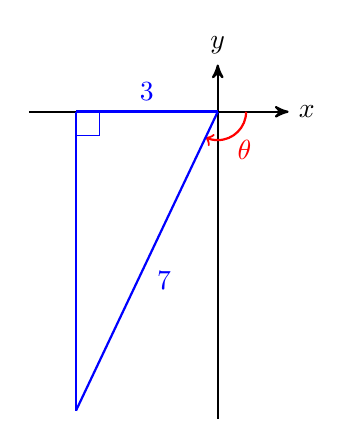
\begin{tikzpicture} [scale=.6]
\coordinate (O) at (0,0);
\coordinate (A) at ($ sqrt(40)*(0,-1) +(-3,0) $);
\coordinate (B) at (-3,0);
\draw[blue] (B) rectangle ++(.5,-.5);
\draw[black,thick,->,>=stealth'] (-4,0)--(1.5,0) node[right]{$x$};
\draw[black,thick,->,>=stealth'] (0,-6.5)--(0,1) node[above]{$y$};
\draw[red,thick, ->] (0.6,0 ) arc(0:{-90-asin(3/7)}:0.6) node[below right, midway, yshift=2, xshift=-2,] {$\theta$};
\draw[blue,thick] (O)--(A) node[below right,midway,text=blue] {$7$};
\draw[blue,thick] (B)--(A);
\draw[blue,very thick] (O)--(B) node[ above, midway, text=blue] {$3$};
\end{tikzpicture}
\newline

hp8-3-29 sunlight through atmosphere

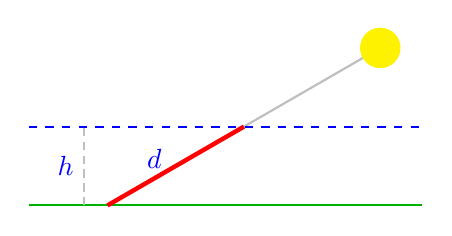
\begin{tikzpicture}
\coordinate (O) at (0,0);
\def\th{30};
\coordinate (S) at ({\th}:4);
\draw[lightgray,thick] (O)--(S);
\filldraw[yellow] (S) circle (.25);
\draw[green!70!black,thick] (-1,0)--(4,0);
\draw[blue, thick, dashed] (-1,1)--(4,1);
\draw[lightgray,thick, densely dashed] (-.3,0)--(-.3,1) node[left,midway, text=blue] {$h$};
\draw[red, ultra thick] (O) -- ($sqrt(3)*(1,0)+(0,1)$) node[above left, xshift=-1, yshift=-5, midway, text=blue] {$d$};
\end{tikzpicture}
\newline


hp8-3-30 railroad track

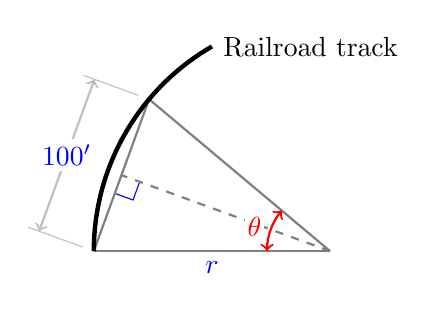
\begin{tikzpicture}
\coordinate (O) at (0,0);
\coordinate (A) at (-3,0);
\def\th{140};
\coordinate (B) at ({\th}:3);
\coordinate (C) at ($ .5*(A)+.5*(B) $);
\coordinate (D) at ($ .12*(B) - .12*(A) $);
\coordinate (E) at ($ -1*(D)+ (C)  $);
\coordinate (F) at ($ (E)+ (O)!-1.0!90:(D)  $);
\coordinate (G) at ($ (F)+ (D)  $);
\coordinate (H) at ($ (O)!3.0!90:(D) $);
\coordinate (P) at ($ (A) +(H)$);
\coordinate (Q) at ($ (B) +(H)$);
\draw[lightgray,thick,<->] (P)--(Q);
\coordinate (R) at ($ .5*(P) +.5*(Q)$);
\node[fill=white, inner sep=2, text=blue] at (R) {$100 '$};
\draw[lightgray] (A)++($ .2*(H) $)--++(H);
\draw[lightgray] (B)++($ .2*(H) $)--++(H);
\draw[blue] (E)--(F)--(G);
\draw[gray,thick] (O)--(A) node[below, midway, text=blue] {$r$};
\draw[gray,thick] (O)--(B)--(A);
\draw[gray,thick, dashed] (O)--(C);
\draw[black,ultra thick] (A) arc(180:120:3) node[right]{Railroad track};
\draw[red,thick, <->] (-.8,0) arc(180:{\th}:.8) node[left, midway, xshift=-2, yshift=1, fill=white, inner sep=1] {$\theta$};
\end{tikzpicture}
\newline

hp8-3-31 inclined plane

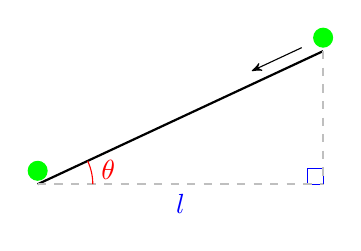
\begin{tikzpicture}
\def\th{25};
\coordinate (O) at (0,0);
\coordinate (A) at ({\th}:4);
\coordinate (B) at ($ 4*cos(\th)*(1,0) $);
\def\ra{0.12};
\def\rb{\ra+\ra*sin(\th)};
\draw[blue] (B) rectangle ++(-.2,.2);
\draw[black,thick] (O)--(A);
\draw[lightgray,thick, dashed] (O)--(B) node[below,midway, text=blue] {$l$};
\draw[lightgray,thick, dashed] (A)--(B);
\filldraw[green] ($ (A)++\rb*(0,1)$) circle ({\ra});
\filldraw[green] ($ (O)++\rb*(0,1)$) circle (\ra cm);
\coordinate (P) at ($ (A) + (\th:-0.3) + \rb*(0,1) $);
\coordinate (Q) at ($ (A) + (\th:-1.) + \rb*(0,1) $);
\draw[black,->,>=stealth'] (P)--(Q);
\draw[red] (0.7,0) arc(0:{\th}:0.7) node[right, midway, yshift=1] {$\theta$};
\end{tikzpicture}
\newline

hp8-3-33 triangle

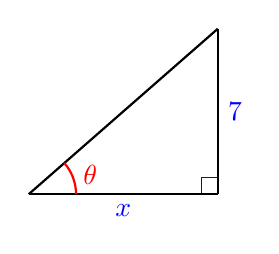
\begin{tikzpicture} [scale=.3]
\coordinate (O) at (0,0);
\coordinate (A) at (8,0);
\coordinate (B) at (8,7);
\draw[blue] (A) rectangle ++(-.7,.7);
\draw[black,thick] (A)--(B) node[right, midway, text=blue]{$7$};
\draw[black,thick] (O)--(A) node[below, midway, text=blue]{$x$};
\draw[black,thick] (O)--(B);
\draw[red,thick] (2,0) arc(0:{atan(7/8)}:2) node[right,yshift=1,midway] {$\theta$};
\end{tikzpicture}
\newline

hp8-3-34 triangle

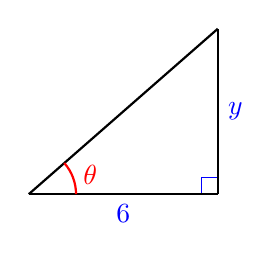
\begin{tikzpicture} [scale=.3]
\coordinate (O) at (0,0);
\coordinate (A) at (8,0);
\coordinate (B) at (8,7);
\draw[blue] (A) rectangle ++(-.7,.7);
\draw[black,thick] (A)--(B) node[right, midway, text=blue]{$y$};
\draw[black,thick] (O)--(A) node[below, midway, text=blue]{$6$};
\draw[black,thick] (O)--(B);
\draw[red,thick] (2,0) arc(0:{atan(7/8)}:2) node[right,yshift=1,midway] {$\theta$};
\end{tikzpicture}
\newline


hp8-3-35 triangle
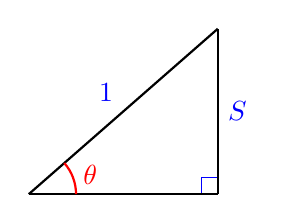
\begin{tikzpicture} [scale=.3]
\coordinate (O) at (0,0);
\coordinate (A) at (8,0);
\coordinate (B) at (8,7);
\draw[blue] (A) rectangle ++(-.7,.7);
\draw[black,thick] (A)--(B) node[right, midway, text=blue]{$S$};
\draw[black,thick] (O)--(A);
\draw[black,thick] (O)--(B) node[above left, midway, text=blue]{$1$};
\draw[red,thick] (2,0) arc(0:{atan(7/8)}:2) node[right,yshift=1,midway] {$\theta$};
\end{tikzpicture}
\newline


hp8-3-36 triangle
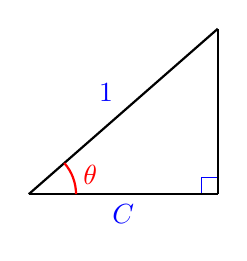
\begin{tikzpicture} [scale=.3]
\coordinate (O) at (0,0);
\coordinate (A) at (8,0);
\coordinate (B) at (8,7);
\draw[blue] (A) rectangle ++(-.7,.7);
\draw[black,thick] (A)--(B);
\draw[black,thick] (O)--(A) node[below, midway, text=blue]{$C$};
\draw[black,thick] (O)--(B) node[above left, midway, text=blue]{$1$};
\draw[red,thick] (2,0) arc(0:{atan(7/8)}:2) node[right,yshift=1,midway] {$\theta$};
\end{tikzpicture}
\newline


hp8-3-37 angle

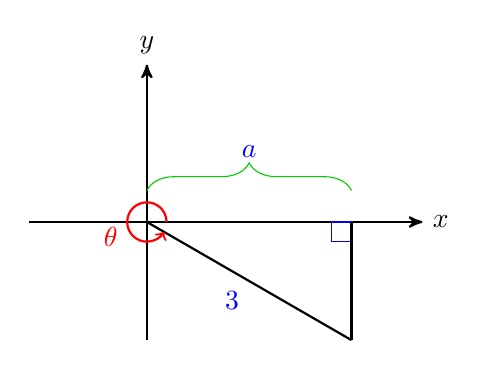
\begin{tikzpicture}
\draw[black,thick,->,>=stealth'] (-1.5,0)--(3.5,0) node[right]{$x$};
\draw[black,thick,->,>=stealth'] (0,-1.5)--(0,2) node[above]{$y$};
\def\th{30};
\coordinate (O) at (0,0);
\coordinate (A) at ($ 3*cos(\th)*(1,0) $);
\coordinate (B) at ({-\th}:3);
\draw[blue] (A) rectangle ++(-.25,-.25);
\draw [green!80!black, decorate, decoration={brace,amplitude=10pt}]
(0.,.4) -- ($ (A)+(0,.4) $) node [blue,above,midway, yshift=.3cm] 
{ $a$};
\draw[black,thick] (O)--(B) node[below left, midway, text=blue] {$3$};
\draw[black,thick] (A)--(B);
\draw[red,thick, ->] (.25,0) arc(0:{360-\th}:0.25) node[below left, midway] {$\theta$};
\end{tikzpicture}
\newline


hp8-3-38 angle

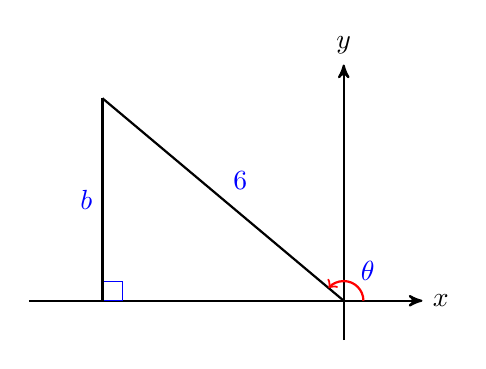
\begin{tikzpicture}
\draw[black,thick,->,>=stealth'] (-4,0)--(1.,0) node[right]{$x$};
\draw[black,thick,->,>=stealth'] (0,-.5)--(0,3) node[above]{$y$};
\def\th{40};
\coordinate (O) at (0,0);
\coordinate (A) at ($ -4*cos(\th)*(1,0) $);
\coordinate (B) at ({180-\th}:4);
\draw[blue] (A) rectangle ++(.25,.25);
\draw[black,thick] (O)--(B) node[above right, midway, text=blue] {$6$};
\draw[black,thick] (A)--(B) node[left, midway, text=blue] {$b$};
\draw[red,thick, ->] (.25,0) arc(0:{180-\th}:0.25) node[above right, yshift=-3, midway, text=blue] {$\theta$};
\end{tikzpicture}
\newline

hp8-3-39 unit circle

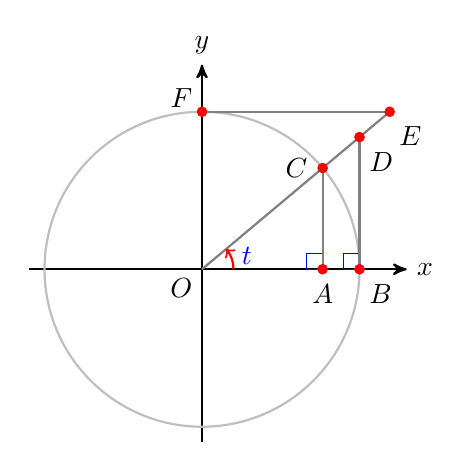
\begin{tikzpicture} [scale=2]
\draw[black,thick,->,>=stealth'] (-1.1,0)--(1.3,0) node[right]{$x$};
\draw[black,thick,->,>=stealth'] (0,-1.1)--(0,1.3) node[above]{$y$};
\def\th{40};
\coordinate (O) at (0,0);
\draw[lightgray,thick] (O) circle (1cm);
\coordinate (A) at ($ cos(\th)*(1,0) $);
\coordinate (B) at (1,0);
\coordinate (C) at ({\th}:1);
\coordinate (D) at ($ tan(\th)*(0,1)+(1,0) $);
\coordinate (E) at ($ cot(\th)*(1,0)+(0,1) $);
\coordinate (F) at (0,1);

\draw[blue] (A) rectangle ++(-.1,.1);
\draw[blue] (B) rectangle ++(-.1,.1);
\draw[gray,thick] (O)--(E);
\draw[gray,thick] (A)--(C);
\draw[gray,thick] (D)--(B);
\draw[gray,thick] (E)--(F);
\draw[red,thick, ->] (.2,0) arc(0:{\th}:0.2) node[right, yshift=1, midway, text=blue] {$t$};
\filldraw[red] (A) circle (.03cm) node[below, yshift=-2, text=black] {$A$};
\filldraw[red] (B) circle (.03cm) node[below right, yshift=-2, text=black] {$B$};
\filldraw[red] (C) circle (.03cm) node[left, xshift=-2, text=black] {$C$};
\filldraw[red] (D) circle (.03cm) node[below right, yshift=-2, text=black] {$D$};
\filldraw[red] (E) circle (.03cm) node[below right, yshift=-2, text=black] {$E$};
\filldraw[red] (F) circle (.03cm) node[above left, yshift=-2, text=black] {$F$};
\node[below left] at (O) {$O$};
\end{tikzpicture}
\newline

hp8-3-41ans angle
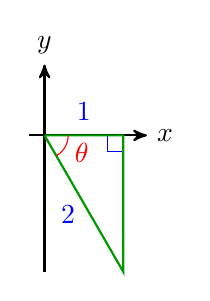
\begin{tikzpicture}
\draw[black,thick,->,>=stealth'] (-.2,0)--(1.3,0) node[right]{$x$};
\draw[black,thick,->,>=stealth'] (0,-1.732)--(0,0.9) node[above]{$y$};
\coordinate (O) at (0,0);
\coordinate (A) at (1,{-sqrt(3)});
\coordinate (B) at (1,0);
\draw[blue] (B) rectangle ++(-.2,-.2);
\draw[green!60!black, thick] (O)--(A)--(B)--(O);
\node[text=blue] at (0.5,0.3) {$1$};
\node[text=blue] at (0.3,-1.) {$2$};
\draw[red] (0.3,0) arc(0:-60:0.3) node[right, midway, yshift=-2] {$\theta$};
\end{tikzpicture}
\newline

hp8-3-43ans angle
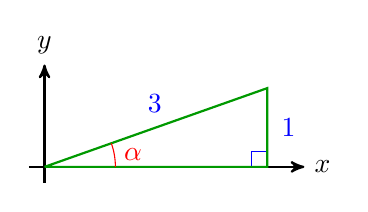
\begin{tikzpicture}
\draw[black,thick,->,>=stealth'] (-.2,0)--(3.3,0) node[right]{$x$};
\draw[black,thick,->,>=stealth'] (0,-.2)--(0,1.3) node[above]{$y$};
\coordinate (O) at (0,0);
\coordinate (A) at ({2*sqrt(2)},1);
\coordinate (B) at ({sqrt(8)},0);
\draw[blue] (B) rectangle ++(-.2,.2);
\draw[green!60!black, thick] (O)--(A)--(B)--(O);
\node[text=blue] at (1.4,0.8) {$3$};
\node[text=blue] at (3.1,.5) {$1$};
\draw[red] (0.9,0) arc(0:{asin(1/3)}:0.9) node[right, midway, yshift=0] {$\alpha$};
\end{tikzpicture}
\newline

hp8-3-45ans angle
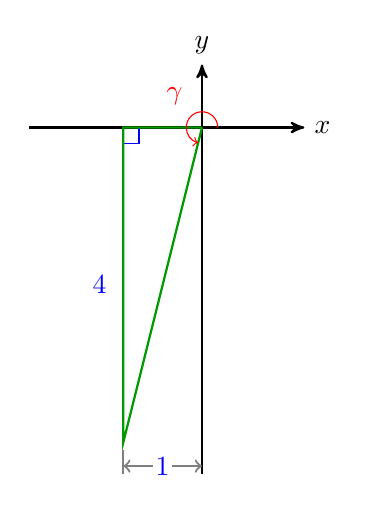
\begin{tikzpicture}
\draw[black,thick,->,>=stealth'] (-2.2,0)--(1.3,0) node[right]{$x$};
\draw[black,thick,->,>=stealth'] (0,-4.4)--(0,0.8) node[above]{$y$};
\coordinate (O) at (0,0);
\coordinate (A) at (-1,-4);
\coordinate (B) at (-1,0);
\draw[blue] (B) rectangle ++(.2,-.2);
\draw[green!60!black, thick] (O)--(A)--(B)--(O);
\node[text=blue] at (-1.3,-2) {$4$};
\draw[gray,thick] (-1,-4.4)--++(0,.3);
\draw[gray,thick,<->] (-1,-4.3)--++(1,0) node[midway, fill=white, inner sep=1, text=blue] {$1$};
\draw[red,->] (0.2,0) arc(0:{180+atan(4)}:0.2) node[above left, midway, yshift=0] {$\gamma$};
\end{tikzpicture}
\newline


hp8-3-53 grid

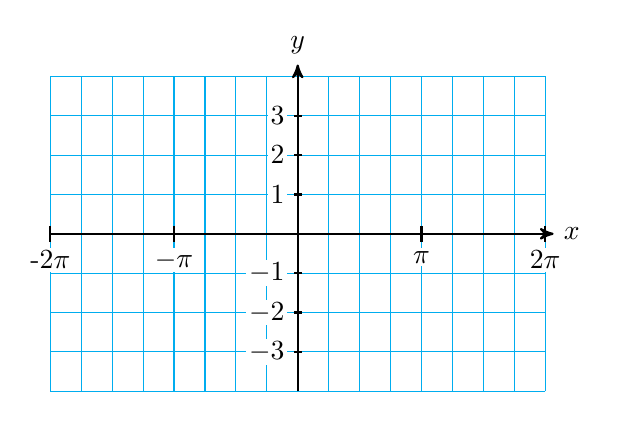
\begin{tikzpicture} [scale=.5]
\draw[cyan] (-2*pi,-4) grid[xstep=pi/4] (2*pi,4);
\draw[black,thick,->,>=stealth'] (-2*pi,0)--(6.5,0) node[right]{$x$};
\draw[black,thick,->,>=stealth'] (0,-4)--(0,4.3) node[above]{$y$};
\foreach \y in {-3,-2,-1,1,2,3} \draw[black,thick] (.1,\y)--++(-.2,0) node [left, xshift=-2, fill=white, inner sep=1] {$\y$};
\draw[black,thick] (-2*pi,.2)--++(0,-.4) node[below, yshift=-2, fill=white, inner sep=1] {-$2\pi$};
\draw[black,thick] (-pi,.2)--++(0,-.4) node[below, yshift=-2, fill=white, inner sep=1] {$-\pi$};
\draw[black,thick] (pi,.2)--++(0,-.4) node[below, yshift=-2, fill=white, inner sep=1] {$\pi$};
\draw[black,thick] (2*pi,.2)--++(0,-.4) node[below, yshift=-2, fill=white, inner sep=1] {$2\pi$};
\end{tikzpicture}
\newline


hp8-3-53ans sec x

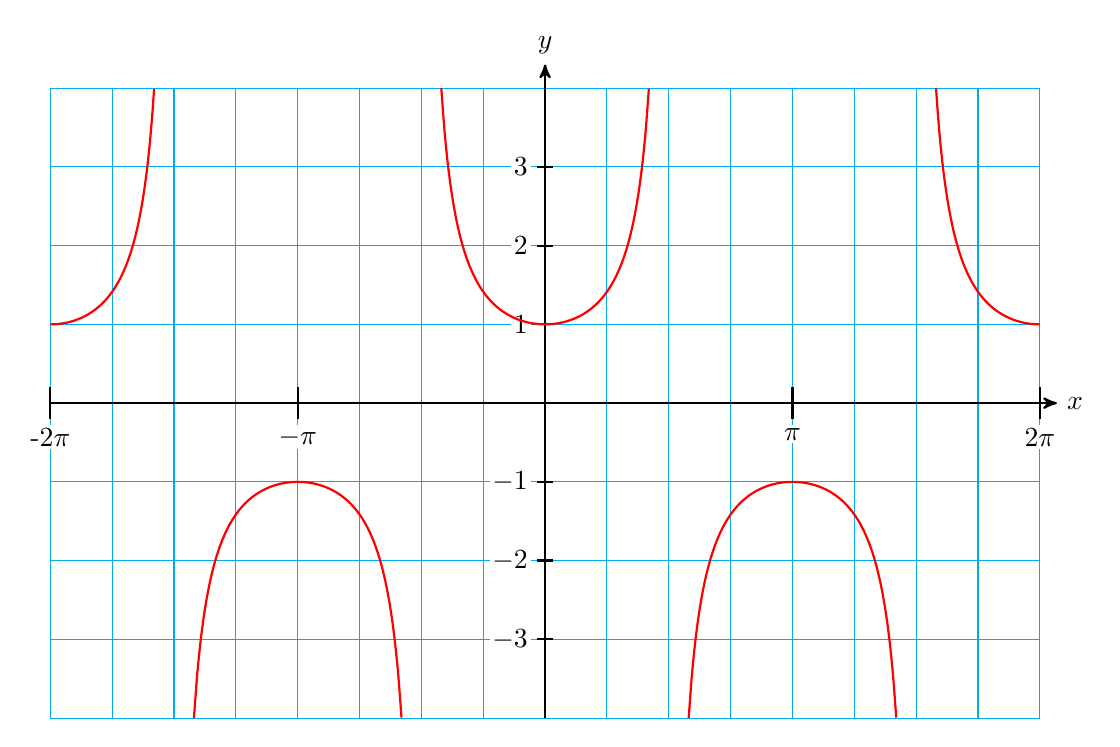
\begin{tikzpicture} scale=.5]
\draw[cyan] (-2*pi,-4) grid[xstep=pi/4] (2*pi,4);
\draw[black,thick,->,>=stealth'] (-2*pi,0)--(6.5,0) node[right]{$x$};
\draw[black,thick,->,>=stealth'] (0,-4)--(0,4.3) node[above]{$y$};
\foreach \y in {-3,-2,-1,1,2,3} \draw[black,thick] (.1,\y)--++(-.2,0) node [left, xshift=-2, fill=white, inner sep=1] {$\y$};
\draw[black,thick] (-2*pi,.2)--++(0,-.4) node[below, yshift=-2, fill=white, inner sep=1] {-$2\pi$};
\draw[black,thick] (-pi,.2)--++(0,-.4) node[below, yshift=-2, fill=white, inner sep=1] {$-\pi$};
\draw[black,thick] (pi,.2)--++(0,-.4) node[below, yshift=-2, fill=white, inner sep=1] {$\pi$};
\draw[black,thick] (2*pi,.2)--++(0,-.4) node[below, yshift=-2, fill=white, inner sep=1] {$2\pi$};
\draw[samples=65, domain={0}:{acos(1/4)*pi/180}, variable=\x, smooth, red, thick] plot ({\x-2*pi}, {sec(deg(\x))});
\draw[samples=65, domain={-acos(1/4)*pi/180}:{acos(1/4)*pi/180}, variable=\x, smooth, red, thick] plot ({\x-pi}, {-sec(deg(\x))});
\draw[samples=65, domain={-acos(1/4)*pi/180}:{acos(1/4)*pi/180}, variable=\x, smooth, red, thick] plot (\x, {sec(deg(\x))});
\draw[samples=65, domain={-acos(1/4)*pi/180}:{acos(1/4)*pi/180}, variable=\x, smooth, red, thick] plot ({\x+pi}, {-sec(deg(\x))});
\draw[samples=65, domain={-acos(1/4)*pi/180}:{0}, variable=\x, smooth, red, thick] plot ({\x+2*pi}, {sec(deg(\x))});
\end{tikzpicture}
\newline

hp8-3-55 sine

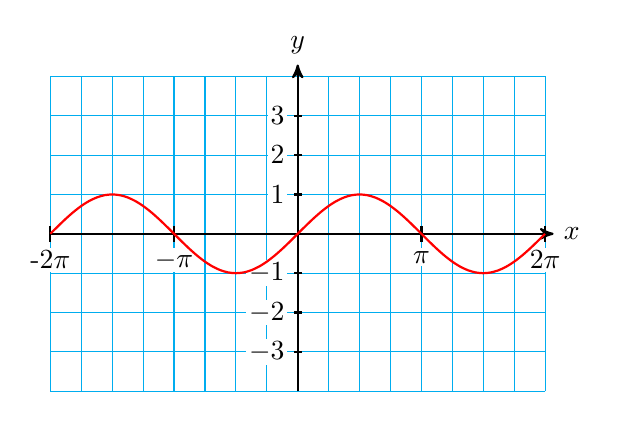
\begin{tikzpicture} [scale=.5]
\draw[cyan] (-2*pi,-4) grid[xstep=pi/4] (2*pi,4);
\draw[black,thick,->,>=stealth'] (-2*pi,0)--(6.5,0) node[right]{$x$};
\draw[black,thick,->,>=stealth'] (0,-4)--(0,4.3) node[above]{$y$};
\foreach \y in {-3,-2,-1,1,2,3} \draw[black,thick] (.1,\y)--++(-.2,0) node [left, xshift=-2, fill=white, inner sep=1] {$\y$};
\draw[black,thick] (-2*pi,.2)--++(0,-.4) node[below, yshift=-2, fill=white, inner sep=1] {-$2\pi$};
\draw[black,thick] (-pi,.2)--++(0,-.4) node[below, yshift=-2, fill=white, inner sep=1] {$-\pi$};
\draw[black,thick] (pi,.2)--++(0,-.4) node[below, yshift=-2, fill=white, inner sep=1] {$\pi$};
\draw[black,thick] (2*pi,.2)--++(0,-.4) node[below, yshift=-2, fill=white, inner sep=1] {$2\pi$};
\draw[samples=65, domain=-2*pi:2*pi, variable=\x, smooth, red, thick] plot (\x,{sin(deg(\x))});
\end{tikzpicture}
\newline

hp8-3-55ans sine and cosecant

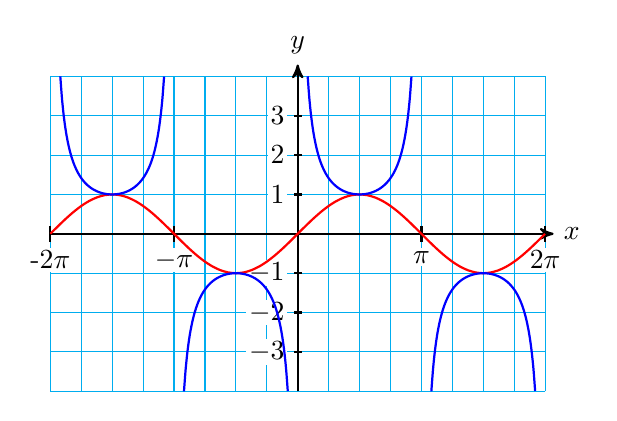
\begin{tikzpicture} [scale=.5]
\draw[cyan] (-2*pi,-4) grid[xstep=pi/4] (2*pi,4);
\draw[black,thick,->,>=stealth'] (-2*pi,0)--(6.5,0) node[right]{$x$};
\draw[black,thick,->,>=stealth'] (0,-4)--(0,4.3) node[above]{$y$};
\foreach \y in {-3,-2,-1,1,2,3} \draw[black,thick] (.1,\y)--++(-.2,0) node [left, xshift=-2, fill=white, inner sep=1] {$\y$};
\draw[black,thick] (-2*pi,.2)--++(0,-.4) node[below, yshift=-2, fill=white, inner sep=1] {-$2\pi$};
\draw[black,thick] (-pi,.2)--++(0,-.4) node[below, yshift=-2, fill=white, inner sep=1] {$-\pi$};
\draw[black,thick] (pi,.2)--++(0,-.4) node[below, yshift=-2, fill=white, inner sep=1] {$\pi$};
\draw[black,thick] (2*pi,.2)--++(0,-.4) node[below, yshift=-2, fill=white, inner sep=1] {$2\pi$};
\draw[samples=65, domain=-2*pi:2*pi, variable=\x, smooth, red, thick] plot (\x,{sin(deg(\x))});
\draw[samples=65, domain={asin(1/4)*pi/180}:{pi-asin(1/4)*pi/180}, variable=\x, smooth, blue, thick] plot (\x, {cosec(deg(\x))});
\draw[samples=65, domain={asin(1/4)*pi/180}:{pi-asin(1/4)*pi/180}, variable=\x, smooth, blue, thick] plot ({\x-2*pi}, {cosec(deg(\x))});
\draw[samples=65, domain={asin(1/4)*pi/180}:{pi-asin(1/4)*pi/180}, variable=\x, smooth, blue, thick] plot ({\x-pi}, {-cosec(deg(\x))});
\draw[samples=65, domain={asin(1/4)*pi/180}:{pi-asin(1/4)*pi/180}, variable=\x, smooth, blue, thick] plot ({\x+pi}, {-cosec(deg(\x))});

\end{tikzpicture}
\newline

hp8-3-56 cosine

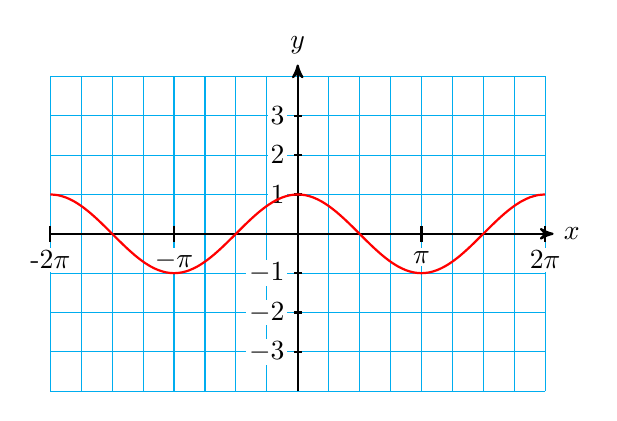
\begin{tikzpicture} [scale=.5]
\draw[cyan] (-2*pi,-4) grid[xstep=pi/4] (2*pi,4);
\draw[black,thick,->,>=stealth'] (-2*pi,0)--(6.5,0) node[right]{$x$};
\draw[black,thick,->,>=stealth'] (0,-4)--(0,4.3) node[above]{$y$};
\foreach \y in {-3,-2,-1,1,2,3} \draw[black,thick] (.1,\y)--++(-.2,0) node [left, xshift=-2, fill=white, inner sep=1] {$\y$};
\draw[black,thick] (-2*pi,.2)--++(0,-.4) node[below, yshift=-2, fill=white, inner sep=1] {-$2\pi$};
\draw[black,thick] (-pi,.2)--++(0,-.4) node[below, yshift=-2, fill=white, inner sep=1] {$-\pi$};
\draw[black,thick] (pi,.2)--++(0,-.4) node[below, yshift=-2, fill=white, inner sep=1] {$\pi$};
\draw[black,thick] (2*pi,.2)--++(0,-.4) node[below, yshift=-2, fill=white, inner sep=1] {$2\pi$};
\draw[samples=65, domain=-2*pi:2*pi, variable=\x, smooth, red, thick] plot (\x,{cos(deg(\x))});
\end{tikzpicture}
\newline

hp8-3-57ans cotangent

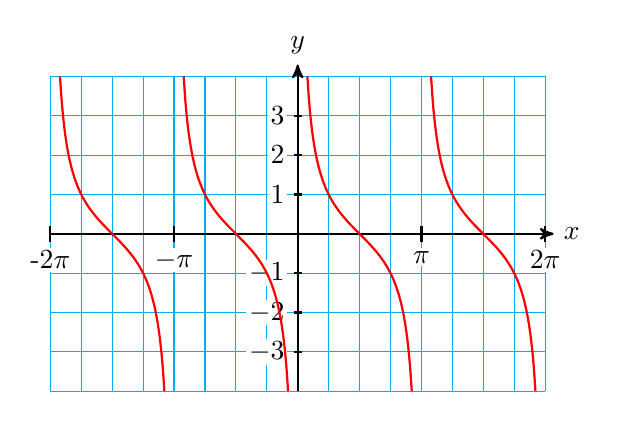
\begin{tikzpicture} [scale=.5]
\draw[cyan] (-2*pi,-4) grid[xstep=pi/4] (2*pi,4);
\draw[black,thick,->,>=stealth'] (-2*pi,0)--(6.5,0) node[right]{$x$};
\draw[black,thick,->,>=stealth'] (0,-4)--(0,4.3) node[above]{$y$};
\foreach \y in {-3,-2,-1,1,2,3} \draw[black,thick] (.1,\y)--++(-.2,0) node [left, xshift=-2, fill=white, inner sep=1] {$\y$};
\draw[black,thick] (-2*pi,.2)--++(0,-.4) node[below, yshift=-2, fill=white, inner sep=1] {-$2\pi$};
\draw[black,thick] (-pi,.2)--++(0,-.4) node[below, yshift=-2, fill=white, inner sep=1] {$-\pi$};
\draw[black,thick] (pi,.2)--++(0,-.4) node[below, yshift=-2, fill=white, inner sep=1] {$\pi$};
\draw[black,thick] (2*pi,.2)--++(0,-.4) node[below, yshift=-2, fill=white, inner sep=1] {$2\pi$};
\draw[samples=65, domain={-atan(4)*pi/180}:{atan(4)*pi/180}, variable=\x, smooth, red, thick] plot ({\x-3*pi/2}, {-tan(deg(\x))});
\draw[samples=65, domain={-atan(4)*pi/180}:{atan(4)*pi/180}, variable=\x, smooth, red, thick] plot ({\x-pi/2}, {-tan(deg(\x))});
\draw[samples=65, domain={-atan(4)*pi/180}:{atan(4)*pi/180}, variable=\x, smooth, red, thick] plot ({\x+pi/2}, {-tan(deg(\x))});
\draw[samples=65, domain={-atan(4)*pi/180}:{atan(4)*pi/180}, variable=\x, smooth, red, thick] plot ({\x+3*pi/2}, {-tan(deg(\x))});
\end{tikzpicture}
\newline

hp8-3-58 cosine and sine

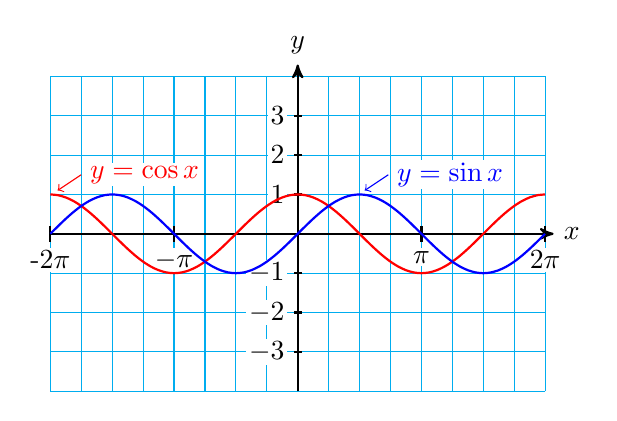
\begin{tikzpicture} [scale=.5]
\draw[cyan] (-2*pi,-4) grid[xstep=pi/4] (2*pi,4);
\draw[black,thick,->,>=stealth'] (-2*pi,0)--(6.5,0) node[right]{$x$};
\draw[black,thick,->,>=stealth'] (0,-4)--(0,4.3) node[above]{$y$};
\foreach \y in {-3,-2,-1,1,2,3} \draw[black,thick] (.1,\y)--++(-.2,0) node [left, xshift=-2, fill=white, inner sep=1] {$\y$};
\draw[black,thick] (-2*pi,.2)--++(0,-.4) node[below, yshift=-2, fill=white, inner sep=1] {-$2\pi$};
\draw[black,thick] (-pi,.2)--++(0,-.4) node[below, yshift=-2, fill=white, inner sep=1] {$-\pi$};
\draw[black,thick] (pi,.2)--++(0,-.4) node[below, yshift=-2, fill=white, inner sep=1] {$\pi$};
\draw[black,thick] (2*pi,.2)--++(0,-.4) node[below, yshift=-2, fill=white, inner sep=1] {$2\pi$};
\draw[samples=65, domain=-2*pi:2*pi, variable=\x, smooth, red, thick] plot (\x,{cos(deg(\x))});
\draw[red,<-,=stealth'] (-6.1,1.1)--++(.6,.4) node[right,xshift=2, fill=white, inner sep=1] {$y=\cos x$};
\draw[samples=65, domain=-2*pi:2*pi, variable=\x, smooth, blue, thick] plot (\x,{sin(deg(\x))});
\draw[blue,<-,=stealth'] (1.7,1.1)--++(.6,.4) node[right,xshift=2, fill=white, inner sep=1] {$y=\sin x$};
\end{tikzpicture}
\newline

hp8-3-77 unit circle

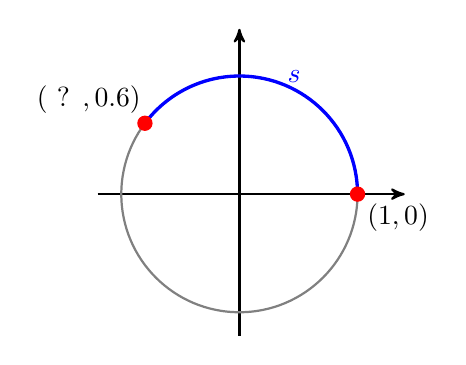
\begin{tikzpicture} [scale=1.5]
\draw[black,thick,->,>=stealth'] (-1.2,0)--(1.4,0);
\draw[black,thick,->,>=stealth'] (0,-1.2)--(0,1.4);
\draw[gray,thick] (0,0) circle (1cm);
\coordinate (A) at (1,0);
\coordinate (B) at (-0.8,0.6);
\draw[blue, very thick] (1,0) arc(0:{acos(-4/5)}:1) node[right, yshift=2, midway] {$s$};
\filldraw[red] (A) circle (.06cm) node[below right, text=black] {$(1,0)$};
\filldraw[red] (B) circle (.06cm) node[above left, xshift=2, text=black] {$($ ? $,0.6)$};
\end{tikzpicture}
\newline

hp8-3-78 unit circle

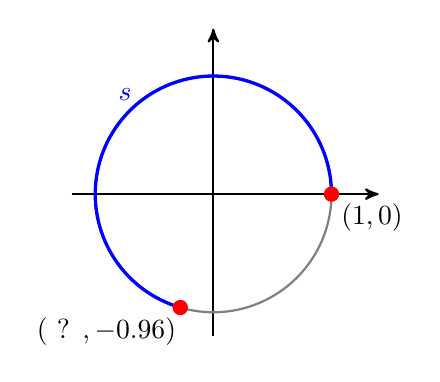
\begin{tikzpicture} [scale=1.5]
\draw[black,thick,->,>=stealth'] (-1.2,0)--(1.4,0);
\draw[black,thick,->,>=stealth'] (0,-1.2)--(0,1.4);
\draw[gray,thick] (0,0) circle (1cm);
\coordinate (A) at (1,0);
\coordinate (B) at ({180+asin(0.96)}:1);
\draw[blue, very thick] (1,0) arc(0:{180+asin(0.96)}:1) node[left, yshift=2, midway] {$s$};
\filldraw[red] (A) circle (.06cm) node[below right, text=black] {$(1,0)$};
\filldraw[red] (B) circle (.06cm) node[below left, xshift=2, text=black] {$($ ? $, -0.96)$};
\end{tikzpicture}
\newline

hp8-3-79 unit circle

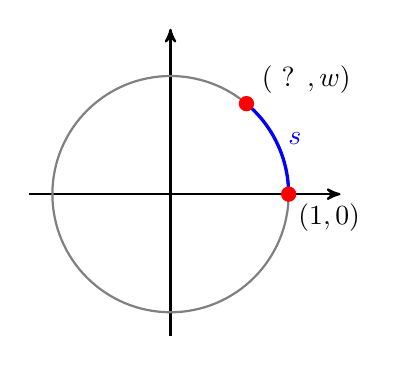
\begin{tikzpicture} [scale=1.5]
\draw[black,thick,->,>=stealth'] (-1.2,0)--(1.44,0);
\draw[black,thick,->,>=stealth'] (0,-1.2)--(0,1.4);
\draw[gray,thick] (0,0) circle (1cm);
\coordinate (A) at (1,0);
\coordinate (B) at (50:1);
\draw[blue, very thick] (1,0) arc(0:50:1) node[right, yshift=2, midway] {$s$};
\filldraw[red] (A) circle (.06cm) node[below right, text=black] {$(1,0)$};
\filldraw[red] (B) circle (.06cm) node[above right, xshift=2, text=black] {$($ ? $, w)$};
\end{tikzpicture}
\newline

hp8-3-80 unit circle

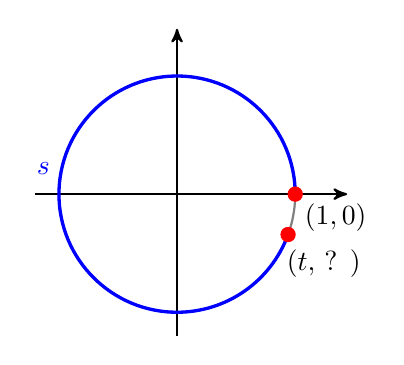
\begin{tikzpicture} [scale=1.5]
\draw[black,thick,->,>=stealth'] (-1.2,0)--(1.44,0);
\draw[black,thick,->,>=stealth'] (0,-1.2)--(0,1.4);
\draw[gray,thick] (0,0) circle (1cm);
\coordinate (A) at (1,0);
\coordinate (B) at (340:1);
\draw[blue, very thick] (1,0) arc(0:340:1) node[left, yshift=2, midway] {$s$};
\filldraw[red] (A) circle (.06cm) node[below right, text=black] {$(1,0)$};
\filldraw[red] (B) circle (.06cm) node[below right, xshift=-4, yshift=-2, text=black] {$(t, $ ? $)$};
\end{tikzpicture}
\newline


hp8-3-96 unit circle and trig ratios

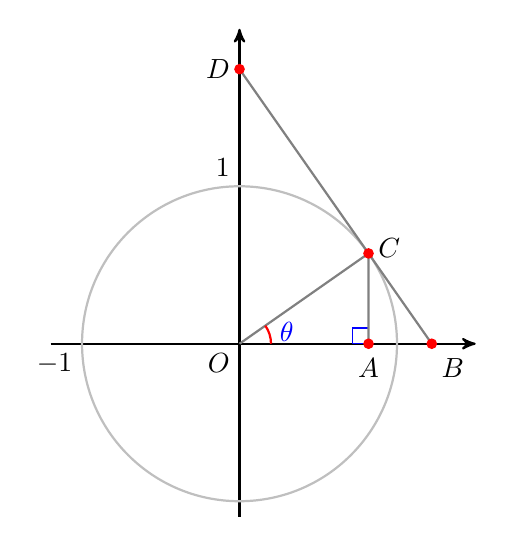
\begin{tikzpicture} [scale=2]
\draw[black,thick,->,>=stealth'] (-1.2,0)--(1.5,0);
\draw[black,thick,->,>=stealth'] (0,-1.1)--(0,2);
\def\th{35};
\coordinate (O) at (0,0);
\draw[lightgray,thick] (O) circle (1cm);
\coordinate (A) at ($ cos(\th)*(1,0) $);
\coordinate (B) at ($ 1/cos(\th)*(1,0) $);
\coordinate (C) at ({\th}:1);
\coordinate (D) at ($ 1/sin(\th)*(0,1) $);

\draw[blue] (A) rectangle ++(-.1,.1);
\draw[gray,thick] (A)--(C)--(O);
\draw[gray,thick] (D)--(B);
\draw[red,thick] (.2,0) arc(0:{\th}:0.2) node[right, yshift=1, midway, text=blue] {$\theta$};
\filldraw[red] (A) circle (.03cm) node[below, yshift=-2, text=black] {$A$};
\filldraw[red] (B) circle (.03cm) node[below right, yshift=-2, text=black] {$B$};
\filldraw[red] (C) circle (.03cm) node[right, yshift=2, text=black] {$C$};
\filldraw[red] (D) circle (.03cm) node[left, text=black] {$D$};
\node[below left] at (O) {$O$};
\node[above left] at (0,1) {$1$};
\node[below left] at (-1,0) {$-1$};

\end{tikzpicture}
\newline

hp8-rev-17 3-4-5 triangle

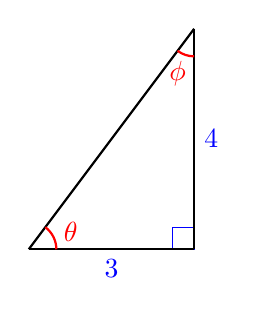
\begin{tikzpicture} [scale=.7]
\coordinate (O) at (0,0);
\coordinate (A) at (3,0);
\coordinate (B) at (3,4);
\draw[blue] (A) rectangle ++(-.4,.4);
\draw[black,thick] (O)--(A) node[below, midway, text=blue] {$3$};
\draw[black,thick] (B)--(A) node[right, midway, text=blue] {$4$};
\draw[black,thick] (O)--(B);
\draw[red,thick] (0.5,0) arc (0:atan(4/3):0.5) node[right, yshift=2, midway] {$\theta$};
\draw[red,thick] (3,3.5) arc (270:{180+atan(4/3)}:0.5) node[below] {$\phi$};
\end{tikzpicture}
\newline

hp8-rev-43 triangle

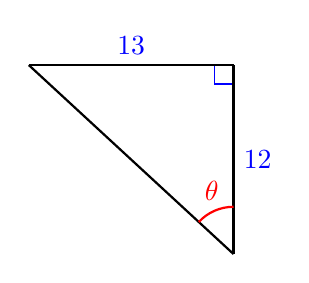
\begin{tikzpicture} [scale=.2]
\coordinate (O) at (0,0);
\coordinate (A) at (13,0);
\coordinate (B) at (13,-12);
\draw[blue] (A) rectangle ++(-1.2,-1.2);
\draw[black,thick] (O)--(A) node[above, midway, text=blue] {$13$};
\draw[black,thick] (B)--(A) node[right, midway, text=blue] {$12$};
\draw[black,thick] (O)--(B);
\draw[red,thick] (13,-9) arc (90:90+atan(13/12):3) node[above, midway, xshift=-1, midway] {$\theta$};
\end{tikzpicture}
\newline

hp8-rev-44 triangle

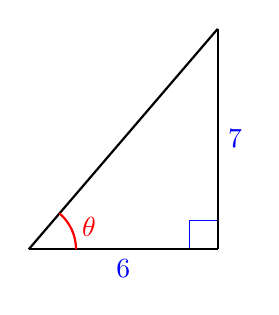
\begin{tikzpicture} [scale=.4]
\coordinate (O) at (0,0);
\coordinate (A) at (6,0);
\coordinate (B) at (6,7);
\draw[blue] (A) rectangle ++(-.9,.9);
\draw[black,thick] (O)--(A) node[below, midway, text=blue] {$6$};
\draw[black,thick] (B)--(A) node[right, midway, text=blue] {$7$};
\draw[black,thick] (O)--(B);
\draw[red,thick] (1.5,0) arc (0:atan(7/6):1.5) node[right, midway, yshift=1, midway] {$\theta$};
\end{tikzpicture}
\newline

hp8-rev-45 triangle

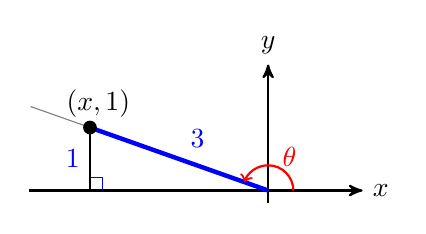
\begin{tikzpicture} [scale=.8]
\draw[black,thick,->,>=stealth'] (-3.8,0)--(1.5,0) node[right] {$x$};
\draw[black,thick,->,>=stealth'] (0,-.2)--(0,2) node[above] {$y$};
\coordinate (O) at (0,0);
\coordinate (A) at ({-sqrt(8)},0);
\coordinate (B) at ({-sqrt(8)},1);
\draw[blue] (A) rectangle ++(.2,.2);
\draw[black,thick] (O)--(A);
\draw[gray] (O)--({180-asin(1/3)}:4);
\draw[black,thick] (B)--(A) node[left, midway, text=blue] {$1$};
\draw[blue, ultra thick] (O)--(B) node[above right, midway, text=blue] {$3$};
\draw[red,thick,->] (0.4,0) arc (0:{180-asin(1/3)}:0.4) node[above right, midway, yshift=-4] {$\theta$};
\filldraw[black] (B) circle (.1cm) node[above, xshift=3] {$(x,1)$};
\end{tikzpicture}
\newline

hp8-rev-46 triangle

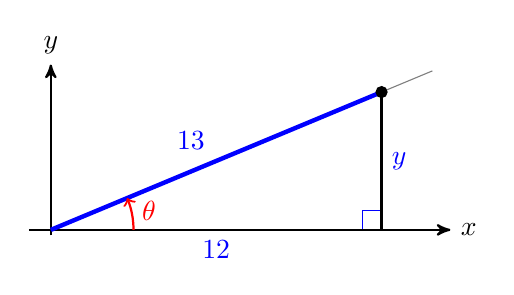
\begin{tikzpicture} [scale=.35]
\draw[black,thick,->,>=stealth'] (-.8,0)--(14.5,0) node[right] {$x$};
\draw[black,thick,->,>=stealth'] (0,-.2)--(0,6) node[above] {$y$};
\coordinate (O) at (0,0);
\coordinate (A) at (12,0);
\coordinate (B) at (12,5);
\draw[blue] (A) rectangle ++(-0.7,0.7);
\draw[black,thick] (O)--(A) node[below, midway, text=blue] {$12$};
\draw[gray] (O)--({acos(12/13)}:15);
\draw[black,thick] (B)--(A) node[right, midway, text=blue] {$y$};
\draw[blue, ultra thick] (O)--(B) node[above left, midway, text=blue] {$13$};
\draw[red,thick,->] (3,0) arc (0:acos(12/13):3) node[right, midway, yshift=1] {$\theta$};
\filldraw[black] (B) circle (.2cm) ;
\end{tikzpicture}
\newline

hp8-rev-47 angle

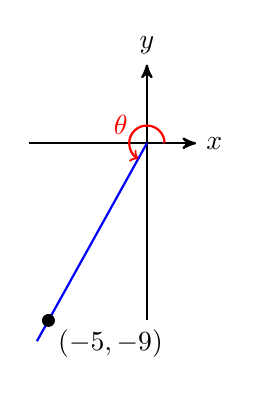
\begin{tikzpicture} [scale=.25]
\draw[black,thick,->,>=stealth'] (-6,0)--(2.5,0) node[right] {$x$};
\draw[black,thick,->,>=stealth'] (0,-9)--(0,4) node[above] {$y$};
\coordinate (O) at (0,0);
\coordinate (A) at (-5,-9);
\draw[blue,thick] (O)--({180+atan(9/5)}:11.5);
\draw[red,thick,->] (.9,0) arc (0:{180+atan(9/5)}:.9) node[left, midway, yshift=1] {$\theta$};
\filldraw[black] (A) circle (.3cm) node[below right] {$(-5,-9)$};
\end{tikzpicture}
\newline

hp8-rev-48 angle

\begin{tikzpicture} [scale=.35]
\draw[black,thick,->,>=stealth'] (-2,0)--(5.9,0) node[right] {$x$};
\draw[black,thick,->,>=stealth'] (0,-9)--(0,2) node[above] {$y$};
\coordinate (O) at (0,0);
\coordinate (A) at (4,-8);
\draw[blue,thick] (O)--({-atan(2)}:10);
\draw[red,thick,->] (.9,0) arc (0:{360-atan(9/5)}:.9) node[left, midway, yshift=-11] {$\theta$};
\filldraw[black] (A) circle (.3cm) node[above right] {$(4,-8)$};
\end{tikzpicture}
\newline

hp8-rev-51 angle

\begin{tikzpicture} 
\draw[black,thick,->,>=stealth'] (-1,0)--(4.5,0) node[right] {$x$};
\draw[black,thick,->,>=stealth'] (0,-1)--(0,2) node[above] {$y$};
\def\th{-335};
\coordinate (O) at (0,0);
\coordinate (A) at ({\th}:4);
\coordinate (B) at ($  4*cos(\th)*(1,0) $);
\draw[blue,thick] (B) rectangle ++(-.25,.25);
\draw[black,thick] (O)--(A) node[above left, midway, text=blue] {$4$};
\draw[black,thick] (B)--(A) node[right, midway, text=blue] {$s$};
\draw[red,thick,->] (.4,0) arc (0:{\th}:.4) node[above left, midway, xshift=2, yshift=3] {$\theta$};
\end{tikzpicture}
\newline

hp8-rev-52 angle

\begin{tikzpicture} [scale=.25]
\draw[black,thick,->,>=stealth'] (-17.2,0)--(3,0) node[right] {$x$};
\draw[black,thick,->,>=stealth'] (0,-7)--(0,3) node[above] {$y$};
\def\th{205};
\coordinate (O) at (0,0);
\coordinate (A) at ($ -7/tan(\th)*(1,0) + (0,-7)$);
\coordinate (B) at ($ -7/tan(\th)*(1,0) $);
\draw[blue,thick] (B) rectangle ++(1,-1);
\draw[gray] (A)++(-0.2,0) -- ++(-2,0);
\draw[gray,<->,>=stealth'] (B)++(-1,0) -- ++(0,-7) node[midway, fill=white, inner sep=2, text=blue]{$7$};
\draw[black,thick] (O)--(A) node[below right, midway, text=blue] {$r$};
\draw[black,thick] (B)--(A);
\draw[red,thick,->] (1,0) arc (0:{\th}:1) node[above left, midway, yshift=-3] {$\theta$};
\end{tikzpicture}
\newline

hp8-rev-53 triangle

\begin{tikzpicture} [scale=.3]
\draw[black,thick,->,>=stealth'] (-13.7,0)--(4,0) node[right] {$x$};
\draw[black,thick,->,>=stealth'] (0,-1.5)--(0,6) node[above] {$y$};
\def\th{145};
\coordinate (O) at (0,0);
\coordinate (A) at ($ -12*tan(\th)*(0,1) + (-12,0)$);
\coordinate (B) at (-12,0);
\draw[blue,thick] (B) rectangle ++(1,1);
\draw[gray] (A)++(-0.2,0) -- ++(-1.7,0);
\draw[gray,<->,>=stealth'] (-13,0) -- ($ (A)+(-1,0) $) node[midway, fill=white, inner sep=2, text=blue]{$w$};
\draw[gray] (-12,-.2) --++(0,-1.3);
\draw[gray,<->,>=stealth'] (-12,-1) --++(12,0) node[midway, fill=white, inner sep=2, text=blue]{$12$};
\draw[black,thick] (O)--(A);
\draw[black,thick] (B)--(A);
\draw[red,thick,->] (1,0) arc (0:{\th}:1) node[above right, midway, yshift=-2, yshift=-3] {$\theta$};
\end{tikzpicture}
\newline


hp8-rev-54 triangle

\begin{tikzpicture} [scale=.6]
\draw[black,thick,->,>=stealth'] (-1,0)--(7.8,0) node[right] {$x$};
\draw[black,thick,->,>=stealth'] (0,-3)--(0,2) node[above] {$y$};
\def\th{335};
\coordinate (O) at (0,0);
\coordinate (A) at ($ -3/tan(\th)*(1,0) + (0,-3)$);
\coordinate (B) at ($ -3/tan(\th)*(1,0) $);
\draw[blue,thick] (B) rectangle ++(-.5,-.5);
\draw[gray] (A)++(0.2,0) -- ++(1.,0);
\draw[gray,<->,>=stealth'] (7,0) -- ++(0,-3) node[midway, fill=white, inner sep=2, text=blue]{$3$};
\coordinate (C) at ($ (B) + (0,1.) $);
\draw[gray] (B)++(0,0.2) --++(0,1.3);
\draw[gray,<->,>=stealth'] (0,1.) --(C) node[midway, fill=white, inner sep=2, text=blue]{$u$};
\draw[black,thick] (O)--(A);
\draw[black,thick] (B)--(A);
\draw[red,thick,->] (.45,0) arc (0:{\th}:.45) node[below left, midway, xshift=2, yshift=-3] {$\theta$};
\end{tikzpicture}
\newline

hp8-rev-57 (non-unit) circle

\begin{tikzpicture} [scale=3.5]
\draw[black,thick,->,>=stealth'] (-0.6,0)--(0.75,0);
\draw[black,thick,->,>=stealth'] (0,-0.6)--(0,.7);
\draw[gray,thick] (0,0) circle (0.5cm);
\coordinate (A) at (1/2,0);
\coordinate (B) at (-0.4, 0.3);
\draw[red, very thick] (A) arc(0:{acos(-4/5)}:1/2) node[above right, xshift=2, yshift=-5, midway] {$\theta$};
\filldraw[black] (A) circle (.02cm) node[below right] {$(0.5,0)$};
\filldraw[black] (B) circle (.02cm) node[above left] {$(-0.4,0.3)$};

\end{tikzpicture}
\newline

hp8-rev-57 unit circle

\begin{tikzpicture} [scale=1.75]
\draw[black,thick,->,>=stealth'] (-1.2,0)--(1.5,0);
\draw[black,thick,->,>=stealth'] (0,-1.2)--(0,1.4);
\draw[gray,thick] (0,0) circle (1cm);
\coordinate (A) at (1,0);
\coordinate (B) at (-0.96, -0.28);
\draw[red, very thick] (A) arc(0:{180+acos(0.96)}:1) node[above left, xshift=-0.5cm, yshift=-.25cm, midway] {$\theta$};
\filldraw[black] (A) circle (.04cm);
\filldraw[black] (B) circle (.04cm) node[below left] {$(-0.96,-0.28)$};

\end{tikzpicture}
\newline

hp8-rev-83 triangles

\begin{tikzpicture} [scale=3.3]
\def\al{50};
\def\be{35};
\coordinate (A) at ($ tan(\al)*(0,1)+(1,0) $);
\coordinate (B) at (0,0);
\coordinate (C) at (1,0);
\coordinate (D) at ($ tan(\be)*(0,1)+(1,0) $);
\draw[blue] (C) rectangle ++(-.08,.08);
\draw[black,thick] (C)--(A)--(B)--(D);
\draw[black,thick] (B)--(C) node[below, midway, text=blue]{$1$};
\draw[red,  thick,->] (0.2,0) arc(0:{\al}:0.2) node[above left, xshift=-0., yshift=0, fill=white, inner sep=1] {$\alpha$};
\draw[red,  thick,->] (0.3,0) arc(0:{\be}:0.3) node[right,midway, xshift=2, yshift=0, fill=white, inner sep=1] {$\beta$};
\filldraw[black] (A) circle (0.02 cm) node[right] {$A$};
\filldraw[black] (B) circle (0.02 cm) node[left] {$B$};
\filldraw[black] (C) circle (0.02 cm) node[below] {$C$};
\filldraw[black] (D) circle (0.02 cm) node[right] {$D$};

%second figure
\def\de{1.7};
\coordinate (A) at ($ \de*(1,0)+ tan(\al)*(0,1)+(1,0) $);
\coordinate (B) at ($ \de*(1,0)+(0,0) $);
\coordinate (C) at ($ \de*(1,0)+(1,0) $);
\coordinate (D) at ($ \de*(1,0)+ tan(\be)*(0,1)+(1,0) $);
\coordinate (F) at ($ (C)+ tan(\al)*tan(\be)*(1,0) $);
\coordinate(E) at ($ (F) + ({90+\al}:1.41)  $);
\draw[blue] (C) rectangle ++(-.08,.08);
\draw[black,thick] (D)--(B)--(A)--(C)--(F)--(E);
\draw[blue,thick] (B)--(C) node[below, midway, text=blue]{$1$};
\draw[red,  thick,->] ($ \de*(1,0)+(0.2,0)$) arc(0:{\al}:0.2) node[above left, xshift=-0., yshift=0, fill=white, inner sep=1] {$\alpha$};
\draw[red,  thick,->] ($ \de*(1,0)+(0.3,0)$) arc(0:{\be}:0.3) node[right,midway, xshift=2, yshift=0, fill=white, inner sep=1] {$\beta$};
\filldraw[black] (A) circle (0.02 cm) node[right] {$A$};
\filldraw[black] (B) circle (0.02 cm) node[left] {$B$};
\filldraw[black] (C) circle (0.02 cm) node[below] {$C$};
\filldraw[black] (D) circle (0.02 cm) node[right] {$D$};

\filldraw[black] (F) circle (0.02 cm) node[below] {$F$};
\filldraw[black] (E) circle (0.02 cm) node[above left] {$E$};
\draw[blue] (E)++({\al}:-.08)-- ++({\al-90}:.08)--++({\al}:.08);

\end{tikzpicture}
\newline

hp8-rev-83b triangles

\begin{tikzpicture} [scale=3]
\def\al{50};
\def\be{35};
\coordinate (A) at ($ tan(\al)*(0,1)+(1,0) $);
\coordinate (B) at (0,0);
\coordinate (C) at (1,0);
\coordinate (D) at ($ tan(\be)*(0,1)+(1,0) $);
\coordinate (F) at ($ (C)+ tan(\al)*tan(\be)*(1,0) $);
\coordinate(E) at ($ (F) + ({90+\al}:1.41)  $);
\draw[blue] (C) rectangle ++(-.08,.08);
\draw[black,thick] (D)--(B)--(A)--(C)--(F)--(E);
\draw[blue,thick] (B)--(C) node[below, midway, text=blue]{$1$};
\draw[red,  thick,->] (0.2,0) arc(0:{\al}:0.2) node[above left, xshift=-0., yshift=0, fill=white, inner sep=1] {$\alpha$};
\draw[red,  thick,->] (0.3,0) arc(0:{\be}:0.3) node[right,midway, xshift=2, yshift=0, fill=white, inner sep=1] {$\beta$};
\filldraw[black] (A) circle (0.02 cm) node[right] {$A$};
\filldraw[black] (B) circle (0.02 cm) node[left] {$B$};
\filldraw[black] (C) circle (0.02 cm) node[below] {$C$};
\filldraw[black] (D) circle (0.02 cm) node[right] {$D$};

\filldraw[black] (F) circle (0.02 cm) node[below] {$F$};
\filldraw[black] (E) circle (0.02 cm) node[above left] {$E$};
\draw[blue] (E)++({\al}:-.08)-- ++({\al-90}:.08)--++({\al}:.08);
\end{tikzpicture}
\newline


hp8-rev-85 circle


\begin{tikzpicture} [scale=.2]
\def\di{25/sin(112)};
\def\ri{25/sin(112)/2};
\coordinate (O) at (0,0);
\coordinate (A) at (45:25);
\def\b{\di *sin(23)};
\coordinate (B) at ($ \b*(1,0) $);

\coordinate(P) at ($ 1/2*(B)$);
\coordinate (Q) at ($(P) + (0,20) $);
\draw [name path=P--Q, opacity=0]  (P) --(Q);
\coordinate(R) at (45:25/2);
\coordinate (S) at ($(R) + (135:10) $);
\draw [name path=R--S, opacity=0]  (R) --(S);
\path [name intersections={of=P--Q and R--S, by=C}];

\draw[gray,thick] (C) circle ({\ri});
\draw[lightgray,thick] (C)++(45:{-\ri})--++(45:{\di}) node[above right, midway, xshift=2, yshift=11, text=blue] {$d$};;
\filldraw[black] (C) circle (0.3cm);

\draw[black,thick] (O)--(B) node[below,midway, yshift=-2, fill=white, inner sep=1, text=blue] {$b$};
\draw[black,thick] (O)--(A) node[above left, yshift=-2,midway, text=blue] {$25$};
\draw[black,thick] (A)--(B) node[right,midway, text=blue] {$a$};
\draw[red] (2,0) arc(0:45:2) node[right, midway, yshift=1] {$\alpha$};
\draw[red] ($ \b*(1,0) - (1.2,0) $) arc(180:58:1.2) node[above left, xshift=2, yshift=-2, midway, scale=.8] {$112\degree$};
\draw[red] ($ (A) + (225:5) $) arc(225:248:5) node[below left, xshift=4, yshift=-2, midway, scale=.8] {$23\degree$};

\end{tikzpicture}
\newline






\end{document}
